% Seminar: Value-at-Risk și Expected Shortfall
% Statistica Piețelor Financiare

\documentclass[9pt, aspectratio=169, t]{beamer}
%=============================================================================
% PREAMBUL COMUN - Statistica Piețelor Financiare
% Versiune robustă pentru macOS (MacTeX / BasicTeX / TeX Live)
% Daniel Traian Pele, Antoaneta Amza - ASE București
%
% MODIFICĂRI față de varianta originală:
%  (1) fontawesome5 făcut OPȚIONAL (\IfFileExists) → nu mai pică dacă lipsește
%  (2) polyglossia cu fallback automat pe babel dacă romanian nu există
%  (3) setmainfont rescris cu Ligatures=TeX și nume normalizate (merge pe macOS)
%  (4) graphicspath extins (include directorul curent + variante relative) ca
%      logo-urile să fie găsite și când lansezi xelatex dintr-un subdirector
%
% Compilare:  xelatex preamble + main, de DOUĂ ori (toc/ref).
%=============================================================================

% Asigură încadrarea conținutului pe diapozitive
\setbeamersize{text margin left=8mm, text margin right=8mm}

%=============================================================================
% CONFIGURARE TEMĂ ȘI STIL
%=============================================================================
\usetheme{default}

% Paletă de Culori
\definecolor{MainBlue}{RGB}{26, 58, 110}
\definecolor{AccentBlue}{RGB}{26, 58, 110}
\definecolor{IDAred}{RGB}{205, 0, 0}
\definecolor{DarkGray}{RGB}{51, 51, 51}
\definecolor{MediumGray}{RGB}{128, 128, 128}
\definecolor{LightGray}{RGB}{248, 248, 248}
\definecolor{VeryLightGray}{RGB}{235, 235, 235}
\definecolor{KeynoteGray}{RGB}{218, 218, 218}
\definecolor{SectionGray}{RGB}{120, 120, 120}
\definecolor{FooterGray}{RGB}{100, 100, 100}
\definecolor{Crimson}{RGB}{220, 53, 69}
\definecolor{Forest}{RGB}{46, 125, 50}
\definecolor{Amber}{RGB}{181, 133, 63}
\definecolor{Orange}{RGB}{230, 126, 34}
\definecolor{Purple}{RGB}{142, 68, 173}

% Fundal gradient (gradient Keynote exact 315°: alb la RGB 218,218,218)
\setbeamertemplate{background}{%
	\begin{tikzpicture}[remember picture, overlay]
		\shade[shading=axis, shading angle=315,
		top color=white, bottom color=KeynoteGray]
		(current page.south west) rectangle (current page.north east);
	\end{tikzpicture}%
}
% Culoare solidă de rezervă pentru compatibilitate
\setbeamercolor{background canvas}{bg=}

\setbeamercolor{palette primary}{bg=MainBlue, fg=white}
\setbeamercolor{palette secondary}{bg=MainBlue!85, fg=white}
\setbeamercolor{palette tertiary}{bg=MainBlue!70, fg=white}
\setbeamercolor{structure}{fg=MainBlue}
\setbeamercolor{title}{fg=IDAred}
\setbeamercolor{frametitle}{fg=IDAred, bg=}
\setbeamercolor{block title}{bg=MainBlue, fg=white}
\setbeamercolor{block body}{bg=VeryLightGray, fg=DarkGray}
\setbeamercolor{block title alerted}{bg=Crimson, fg=white}
\setbeamercolor{block body alerted}{bg=Crimson!8, fg=DarkGray}
\setbeamercolor{block title example}{bg=Forest, fg=white}
\setbeamercolor{block body example}{bg=Forest!8, fg=DarkGray}
\setbeamercolor{item}{fg=MainBlue}

\setbeamerfont{institute}{size=\footnotesize}

\setbeamercolor{author in head/foot}{fg=FooterGray, bg=}
\setbeamercolor{title in head/foot}{fg=FooterGray, bg=}
\setbeamercolor{date in head/foot}{fg=FooterGray, bg=}
\setbeamercolor{section in head/foot}{fg=FooterGray, bg=}
\setbeamercolor{subsection in head/foot}{fg=FooterGray, bg=}

\setbeamertemplate{itemize item}{\color{MainBlue}$\boxdot$}
\setbeamertemplate{itemize subitem}{\color{MainBlue}$\blacktriangleright$}
\setbeamertemplate{itemize subsubitem}{\color{MainBlue}\tiny$\bullet$}
\setbeamertemplate{itemize/enumerate body begin}{\normalsize}
\setbeamertemplate{itemize/enumerate subbody begin}{\normalsize}

\setbeamertemplate{section in toc}{%
	\leavevmode\leftskip=1.5em%
	\llap{\color{MainBlue}$\boxdot$\kern0.5em}%
	\inserttocsection\par%
}

\setlength{\leftmargini}{10pt}
\setlength{\leftmarginii}{10pt}
\makeatletter
\def\@listi{\leftmargin\leftmargini \topsep 0pt \parsep 0pt \itemsep 0pt}
\def\@listii{\leftmargin\leftmarginii \topsep 0pt \parsep 0pt \itemsep 0pt}
\makeatother

\setbeamertemplate{navigation symbols}{}

%=============================================================================
% ANTET PERSONALIZAT
%=============================================================================
\setbeamertemplate{headline}{%
	\vskip10pt%
	\hbox to \paperwidth{%
		\hskip0.5cm%
		{\small\color{FooterGray}\renewcommand{\hyperlink}[2]{##2}\insertsectionhead}%
		\hfill%
		\textcolor{FooterGray}{\small\insertframenumber}%
		\hskip0.5cm%
	}%
	\vskip4pt%
	{\color{FooterGray}\hrule height 0.4pt}%
}

%=============================================================================
% PACHETE — ordine importantă: fontspec ÎNAINTE de polyglossia/babel
%=============================================================================

% --- (1) FONTSPEC + FONTURI ROBUSTE PE macOS ---
\usepackage{fontspec}
% Pe macOS unele fonturi Latin Modern nu sunt înregistrate ca fonturi de sistem.
% Folosim Ligatures=TeX (pentru -- → en-dash etc.) și lăsăm fontspec să caute
% prin kpathsea (merge atât pe Mac, cât și pe Linux/Windows).
\defaultfontfeatures{Ligatures=TeX}
\IfFontExistsTF{Latin Modern Roman}{%
	\setmainfont{Latin Modern Roman}
	\setsansfont{Latin Modern Sans}
	\setmonofont{Latin Modern Mono}
}{%
	% Fallback dacă numele cu spații nu sunt găsite (cazul macOS fără fonturi
	% Latin Modern în /Library/Fonts) — fontspec va folosi fontul implicit.
	\PackageWarning{preamble}{Latin Modern Roman nu a fost gasit; folosesc fontul implicit.}
}

% --- (2) POLYGLOSSIA SAU BABEL CU FALLBACK ---
% Pe versiuni vechi de polyglossia (TeX Live < 2020) limba `romanian` nu există.
% Detectăm și folosim babel ca rezervă.
\IfFileExists{gloss-romanian.ldf}{%
	\usepackage{polyglossia}
	\setdefaultlanguage{romanian}
	\setotherlanguage{english}
}{%
	\PackageWarning{preamble}{polyglossia/romanian indisponibil; folosesc babel.}
	\usepackage[english,romanian]{babel}
}

% --- (3) MATH ȘI GRAFICĂ ---
\usepackage{amsmath, amssymb, amsthm}
\usepackage{mathtools}
\usepackage{bm}
\usepackage{tikz}
\usetikzlibrary{arrows.meta, positioning, shapes, calc, decorations.pathreplacing, shadings}
\usepackage{booktabs}
\usepackage{multirow}
\usepackage{array}
\usepackage{graphicx}
\usepackage{hyperref}
\usepackage{colortbl}
\usepackage{listings}
\lstset{basicstyle=\ttfamily\small, breaklines=true, frame=single, backgroundcolor=\color{VeryLightGray}}
\hypersetup{colorlinks=true, linkcolor=MainBlue, urlcolor=MainBlue}

% --- (4) GRAPHICSPATH cu directorul curent inclus ca fallback ---
\graphicspath{{./}{./logos/}{./charts/}{./photos/}{../logos/}{../charts/}{../photos/}{../../logos/}{../../charts/}{../../photos/}}
\hfuzz=2pt
\vfuzz=2pt

%=============================================================================
% SUBSOL PERSONALIZAT — fontawesome5 făcut OPȚIONAL
%=============================================================================
% Pe BasicTeX / instalări minime de MacTeX, fontawesome5 nu există.
% Dacă lipsește, omitem icoanele (subsolul rămâne curat).
\IfFileExists{fontawesome5.sty}{%
	\usepackage{fontawesome5}
	\newcommand{\hasfontawesome}{true}
}{%
	\PackageWarning{preamble}{fontawesome5 indisponibil; subsolul nu va contine icoane.}
}

\setbeamertemplate{footline}{%
	{\color{FooterGray}\hrule height 0.4pt}%
	\vskip4pt%
	\hbox to \paperwidth{%
		\hskip0.5cm%
		\textcolor{FooterGray}{\small Statistica Piețelor Financiare}%
		\hfill%
		\raisebox{-0.1em}{%
			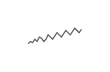
\begin{tikzpicture}[x=0.08em, y=0.08em, line width=0.4pt]
				\draw[FooterGray] (0,3) -- (1,4) -- (2,3.5) -- (3,5) -- (4,4) -- (5,6) -- (6,5.5) -- (7,4) -- (8,5) -- (9,7) -- (10,6) -- (11,5) -- (12,6.5) -- (13,8) -- (14,7) -- (15,6) -- (16,7.5) -- (17,9) -- (18,8) -- (19,7) -- (20,8.5) -- (21,10) -- (22,9) -- (23,8) -- (24,9.5);
			\end{tikzpicture}%
		}%
		\hskip0.5cm%
	}%
	\vskip6pt%
}

%=============================================================================
% COMANDA QUANTLET
%=============================================================================
\newcommand{\quantlet}[2]{%
	\hfill\href{#2}{%
		\raisebox{-0.15em}{
\includegraphics[height=0.7em]{ql_logo.png}}%
		\textcolor{MainBlue}{\tiny\ #1}%
	}%
}

%=============================================================================
% PAGINĂ TITLU PERSONALIZATĂ
%=============================================================================
\defbeamertemplate*{title page}{hybrid}[1][]
{
	\vspace{0.2cm}
	\noindent\makebox[\linewidth][s]{%
		\href{https://www.ase.ro}{
\includegraphics[height=1.0cm]{ase_logo.png}}\hfill%
		\href{https://theida.net}{
\includegraphics[height=1.0cm]{ida_logo.png}}\hfill%
		\href{https://blockchain-research-center.com}{
\includegraphics[height=1.0cm]{brc_logo.png}}\hfill%
		\href{https://www.ai4efin.ase.ro}{
\includegraphics[height=1.0cm]{ai4efin_logo.png}}\hfill%
		\href{https://ipe.ro/new}{
\includegraphics[height=1.0cm]{acad_logo.png}}\hfill%
		\href{https://www.digital-finance-msca.com}{
\includegraphics[height=1.0cm]{msca_logo.png}}%
	}
	\vspace{0.6cm}
	
	\noindent\makebox[\linewidth][c]{%
		\begin{minipage}{0.11\linewidth}
			\centering
			\href{https://quantlet.com}{
\includegraphics[height=1.1cm]{ql_logo.png}}
		\end{minipage}%
		\begin{minipage}{0.76\linewidth}
			\centering
			{\LARGE\bfseries\usebeamercolor[fg]{title}\inserttitle}
			
			\vspace{0.3cm}
			
			{\usebeamerfont{subtitle}\usebeamercolor[fg]{title}\insertsubtitle}
		\end{minipage}%
		\begin{minipage}{0.11\linewidth}
			\centering
			\href{https://quantinar.com}{
\includegraphics[height=1.1cm]{qr_logo.png}}
		\end{minipage}%
	}
	
	\vspace{0.6cm}
	
	\hspace{0.5cm}{\usebeamerfont{author}\insertauthor}
	
	\vspace{0.3cm}
	
	\hspace{0.5cm}\begin{minipage}[t]{0.9\textwidth}
		\raggedright\small\insertinstitute
	\end{minipage}
}
\setbeamertemplate{title page}[hybrid]

%=============================================================================
% MEDII PENTRU TEOREME
%=============================================================================
\theoremstyle{definition}
\setbeamertemplate{theorems}[numbered]
\newtheorem{defn}{Definiție}
\newtheorem{thm}{Teoremă}
\newtheorem{prop}{Propoziție}
\newtheorem{rmk}{Observație}

%=============================================================================
% CENTRED MINIPAGE
%=============================================================================
\newenvironment{cminipage}[1]{%
	\par\noindent\hfill\begin{minipage}{#1}\ignorespaces
	}{%
	\end{minipage}\hfill\null\par
}

%=============================================================================
% COMENZI PERSONALIZATE
%=============================================================================
\newcommand{\E}{\mathbb{E}}
\newcommand{\Var}{\text{Var}}
\newcommand{\Cov}{\text{Cov}}
\newcommand{\Corr}{\text{Corr}}
\newcommand{\VaR}{\text{VaR}}
\newcommand{\ES}{\text{ES}}
\newcommand{\R}{\mathbb{R}}
\newcommand{\N}{\mathbb{N}}
\newcommand{\Z}{\mathbb{Z}}
\newcommand{\B}{\mathbf{B}}
\newcommand{\imark}{\textcolor{MainBlue}{\textbullet}}
\newcommand{\RMSE}{\text{RMSE}}
\newcommand{\MAE}{\text{MAE}}
\newcommand{\MAPE}{\text{MAPE}}
\newcommand{\correct}{\textcolor{Forest}{\checkmark}}
\newcommand{\incorrect}{\textcolor{Crimson}{\texttimes}}

%=============================================================================
% INFORMAȚII TITLU
%=============================================================================
\title[Statistica Piețelor Financiare]{Statistica Piețelor Financiare}
\author[D.T. Pele, A. Amza]{\texorpdfstring{\begin{tabular}[t]{@{}l@{}}Daniel Traian PELE \\ Antoaneta Amza\end{tabular}}{Daniel Traian PELE, Antoaneta Amza}}
\institute{Academia de Studii Economice din București\\
	IDA Institute Digital Assets\\
	Blockchain Research Center\\
	AI4EFin Artificial Intelligence for Energy Finance\\
	Academia Română, Institutul de Prognoză Economică\\
	MSCA Digital Finance}
\date{}
\subtitle{Value-at-Risk și Expected Shortfall}

\begin{document}

%=============================================================================
% PAGINA DE TITLU
%=============================================================================
{
\setbeamertemplate{headline}{}
\setbeamertemplate{footline}{}
\begin{frame}
    \titlepage
\end{frame}
}

%=============================================================================
% CUPRINS SEMINAR
%=============================================================================
\begin{frame}{Cuprins Seminar}
    \begin{cminipage}{0.95\textwidth}
    \begin{itemize}\setlength{\itemsep}{0pt}
        \item \textbf{Recapitulare Rapidă} -- Formule VaR/ES, cele 4 metode, MC, cadrul de reglementare
        \item \textbf{Tehnici Avansate de VaR} -- Cornish-Fisher, FHS, GJR-GARCH, Hill, Block Maxima, LVaR, Lopez
        \item \textbf{Test Grilă} -- 14 întrebări cu variante de răspuns
        \item \textbf{Întrebări Adevărat/Fals} -- 15 întrebări de evaluare conceptuală (3 părți)
        \item \textbf{Exerciții de Calcul} -- 15 probleme rezolvate pas cu pas
        \item \textbf{Studii de caz} -- 7 incidente: Black Monday, Lehman, Crypto, LTCM, COVID, Archegos, UK gilts
        \item \textbf{Exerciții Python} -- 8 exerciții de implementare și backtesting
        \item \textbf{Întrebări de Discuție} -- 6 scenarii (practică, crize, FRTB, crypto, AI, climate)
        \item \textbf{Exerciții cu asistență AI} -- 6 scenarii de gândire critică cu LLM
        \item \textbf{Rezumat} -- Concluzii, temă, glosar, roadmap, bibliografie
    \end{itemize}
    \end{cminipage}
\end{frame}

%=============================================================================
% RECAPITULARE RAPIDĂ
%=============================================================================
\section{Recapitulare Rapidă}

\begin{frame}[shrink=10]{Recapitulare din seminarele anterioare}
    \begin{cminipage}{0.95\textwidth}
    \begin{block}{\faIcon{history} Ce am construit până acum}
    \begin{itemize}\setlength{\itemsep}{0pt}
        \item \textbf{Randamente}: $r_t = \ln(P_t/P_{t-1})$ --- aditive pe orizont
        \item \textbf{Volatilitate}: $\sigma$ măsoară dispersia simetrică, dar \textbf{nu surprinde riscul de coadă}
        \item \textbf{Distribuții cu cozi grele}: Student-$t$, stabile $\alpha$-Lévy --- captează evenimente extreme
        \item \textbf{EVT (POT)}: GPD pe excese peste un prag pentru cuantile foarte mici
    \end{itemize}
    \end{block}
    \vspace{0.1cm}
    \begin{alertblock}{\faIcon{link} Legătura cu seminarul de azi}
    \begin{itemize}\setlength{\itemsep}{0pt}
        \item Azi cuantificăm \textbf{cât pot pierde mâine} la o probabilitate dată: \textbf{VaR}
        \item Și \textbf{cât de mare e pierderea} dacă depășim pragul: \textbf{ES}
        \item Aplicăm cele 4 metode standard (HS, Normal, Student-$t$, MC) și validăm cu \textbf{backtesting}
    \end{itemize}
    \end{alertblock}
    \end{cminipage}
\end{frame}

\begin{frame}[shrink=10]{Formule cheie --- Definiții VaR și ES}
    \begin{cminipage}{0.95\textwidth}
    \begin{columns}[T]
        \begin{column}{0.50\textwidth}
            \textbf{Value-at-Risk (VaR):}
            \begin{itemize}\setlength{\itemsep}{0pt}
                \item Cuantila distribuției pierderilor:
                \[
                \VaR_\alpha = -F_X^{-1}(\alpha) = F_L^{-1}(1-\alpha)
                \]
                \item $X$: rentabilitate; $L = -X$: pierdere
                \item Convenție: $\VaR_{5\%}$ $\equiv$ pierdere depășită cu probabilitate 5\%
                \item Trei elemente: nivel $\alpha$, orizont $h$, distribuție de referință
            \end{itemize}
        \end{column}
        \begin{column}{0.46\textwidth}
            \textbf{Expected Shortfall (ES):}
            \begin{itemize}\setlength{\itemsep}{0pt}
                \item Media pierderilor în coadă:
                \[
                \ES_\alpha = \frac{1}{\alpha}\int_0^\alpha \VaR_u\, du = \E[L \mid L \geq \VaR_\alpha]
                \]
                \item Echivalent (pe rentabilitate):
                \[
                \ES_\alpha = -\E[X \mid X \leq -\VaR_\alpha]
                \]
                \item Mereu $\ES_\alpha \geq \VaR_\alpha$
                \item \textbf{Coerentă} (Acerbi--Tasche); VaR nu este
            \end{itemize}
        \end{column}
    \end{columns}
    \end{cminipage}
\end{frame}

\begin{frame}[shrink=10]{Formule cheie --- Cele 4 metode standard}
    \begin{cminipage}{0.95\textwidth}
    \begin{columns}[T]
        \begin{column}{0.48\textwidth}
            \textbf{1. Simulare istorică (HS):}
            \[
            \widehat{\VaR}_\alpha = -r_{(\lceil \alpha W\rceil)}, \quad
            \widehat{\ES}_\alpha = -\tfrac{1}{\lceil \alpha W\rceil}\textstyle\sum_{i=1}^{\lceil \alpha W\rceil} r_{(i)}
            \]
            cu $r_{(1)} \leq r_{(2)} \leq \cdots \leq r_{(W)}$.

            \vspace{0.15cm}
            \textbf{2. Parametrică Normală:}
            \[
            \VaR_\alpha = -(\mu + \sigma z_\alpha), \quad z_\alpha = \Phi^{-1}(\alpha)
            \]
            \[
            \ES_\alpha = -\mu + \sigma\, \phi(z_\alpha)/\alpha
            \]
        \end{column}
        \begin{column}{0.48\textwidth}
            \textbf{3. Parametrică Student-$t$:}
            \[
            \VaR_\alpha = -\Big(\mu + \sigma\sqrt{\tfrac{\nu-2}{\nu}}\, t_\nu^{-1}(\alpha)\Big)
            \]
            cozi mai grele $\Rightarrow$ $\VaR^{t} > \VaR^{N}$ la $\alpha$ mic.

            \vspace{0.15cm}
            \textbf{4. Monte Carlo:}
            \begin{itemize}\setlength{\itemsep}{0pt}
                \item Simulează $M$ traiectorii ale P\&L
                \item $\widehat{\VaR}_\alpha$ = cuantila empirică $\alpha$
                \item Eroare $\propto 1/\sqrt{M\alpha(1-\alpha)}$
            \end{itemize}

            \vspace{0.15cm}
            \textbf{Scalare orizont:} $\VaR^{(T)} = \sqrt{T}\,\VaR^{(1)}$ (doar sub i.i.d.\ + Normal)
        \end{column}
    \end{columns}
    \end{cminipage}
\end{frame}

\begin{frame}[shrink=10]{Formule cheie --- Backtesting și Basel}
    \begin{cminipage}{0.95\textwidth}
    \begin{columns}[T]
        \begin{column}{0.48\textwidth}
            \textbf{Hit sequence:}
            \[
            I_t = \mathbb{1}\{r_t < -\widehat{\VaR}_\alpha(t)\}
            \]
            Sub model corect: $\E[I_t] = \alpha$, $I_t$ independente.

            \vspace{0.15cm}
            \textbf{Kupiec POF} (acoperire necondițională):
            \[
            LR_{POF} = -2\ln\frac{\alpha^x (1-\alpha)^{n-x}}{\hat p^{\,x}(1-\hat p)^{n-x}} \xrightarrow{H_0} \chi^2_1
            \]
            cu $x = \sum I_t$, $\hat p = x/n$. Respinge dacă $LR > 3{,}84$.
        \end{column}
        \begin{column}{0.48\textwidth}
            \textbf{Christoffersen CC} (acoperire condițională):
            \[
            LR_{CC} = LR_{POF} + LR_{IC} \xrightarrow{H_0} \chi^2_2
            \]

            \vspace{0.15cm}
            \textbf{Basel Traffic Light} ($n=250$, $\alpha=1\%$):
            \begin{center}
            \footnotesize
            \begin{tabular}{lcc}
            \toprule
            \textbf{Zonă} & \textbf{$K$} & \textbf{Add-on} \\
            \midrule
            \textcolor{Forest}{Verde}   & $0$--$4$ & $+0{,}00$ \\
            \textcolor{Amber}{Galben}   & $5$--$9$ & $+0{,}40$--$0{,}85$ \\
            \textcolor{Crimson}{Roșu}   & $\geq 10$ & $+1{,}00$ \\
            \bottomrule
            \end{tabular}
            \end{center}
            Capital: $m \cdot \VaR$, $m = 3 + \text{add-on}$
        \end{column}
    \end{columns}
    \end{cminipage}
\end{frame}

\begin{frame}[shrink=10]{Vizualizare: VaR și ES pe distribuția pierderilor}
    \begin{cminipage}{0.95\textwidth}
    \begin{columns}[T]
    \begin{column}{0.58\textwidth}
    \begin{center}
    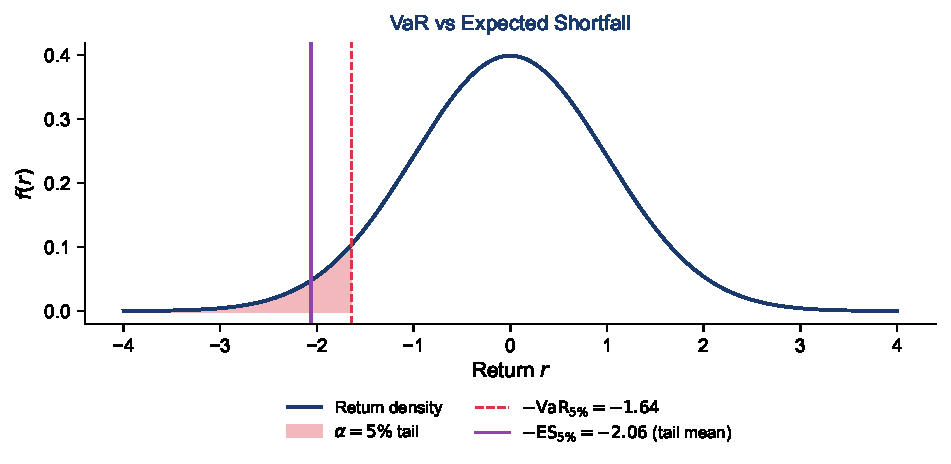
\includegraphics[width=\linewidth]{ch11_var_es_concept.pdf}
    \end{center}
    \end{column}
    \begin{column}{0.40\textwidth}
    \begin{exampleblock}{Citire grafic}
    \begin{itemize}\setlength{\itemsep}{0pt}
        \item \textbf{VaR}: frontiera roșie (cuantila $\alpha$)
        \item \textbf{ES}: media zonei roșii (toate pierderile peste prag)
        \item Sub Normală, $\alpha = 5\%$: $\VaR = 1{,}64\sigma$, $\ES = 2{,}06\sigma$
        \item Sub Normală, $\alpha = 1\%$: $\VaR = 2{,}33\sigma$, $\ES = 2{,}67\sigma$
        \item FRTB: ES~97{,}5\% $\approx$ VaR~99\% sub Normală
    \end{itemize}
    \end{exampleblock}
    \end{column}
    \end{columns}
    \quantlet{SFM\_ch11\_var\_concept}{https://github.com/danpele/SFM/tree/main/Quantlets/Ch_11/SFM_ch11_var_concept}
    \end{cminipage}
\end{frame}

\begin{frame}[shrink=10]{Compararea celor 4 metode pe aceleași date}
    \begin{cminipage}{0.95\textwidth}
    \begin{columns}[T]
    \begin{column}{0.55\textwidth}
    \begin{center}
    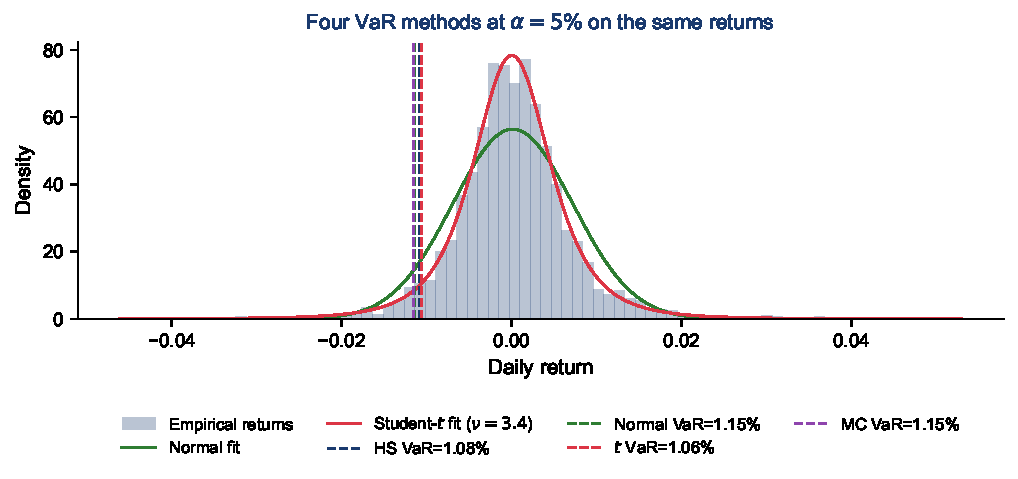
\includegraphics[width=\linewidth]{ch11_methods_comparison.pdf}
    \end{center}
    \end{column}
    \begin{column}{0.43\textwidth}
    \begin{exampleblock}{Observații}
    \begin{itemize}\setlength{\itemsep}{0pt}
        \item Date: 2500 randamente GARCH(1,1)-$t_6$ simulate
        \item Metoda \textbf{Normală} (albastru) \textbf{subestimează} sistematic VaR-ul
        \item \textbf{HS} și \textbf{Student-$t$} converg pe coadă (ambele captează leptokurtoză)
        \item \textbf{MC} cu $M = 10^5$: variabilitate mică pentru $\alpha = 5\%$
        \item Diferențele \textbf{cresc dramatic} la $\alpha = 1\%$ și $0{,}1\%$
    \end{itemize}
    \end{exampleblock}
    \begin{alertblock}{Recomandare}
    \begin{itemize}\setlength{\itemsep}{0pt}
        \item Raportați VaR cu \textbf{mai multe metode} simultan + interval de încredere bootstrap
    \end{itemize}
    \end{alertblock}
    \end{column}
    \end{columns}
    \quantlet{SFM\_ch11\_methods\_comparison}{https://github.com/danpele/SFM/tree/main/Quantlets/Ch_11/SFM_ch11_methods_comparison}
    \end{cminipage}
\end{frame}

\begin{frame}[shrink=10]{Raportul ES/VaR --- cât de important sunt cozile?}
    \begin{cminipage}{0.95\textwidth}
    \begin{columns}[T]
    \begin{column}{0.55\textwidth}
    \begin{center}
    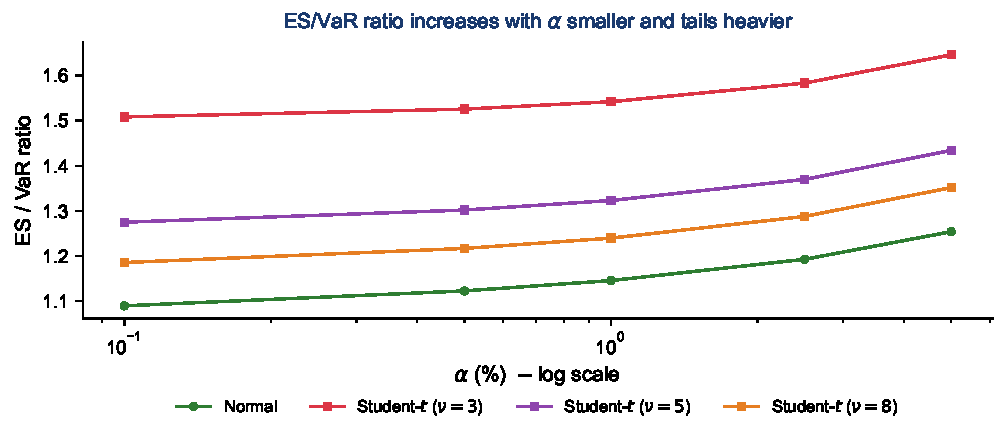
\includegraphics[width=\linewidth]{ch11_es_var_ratio.pdf}
    \end{center}
    \end{column}
    \begin{column}{0.43\textwidth}
    \begin{exampleblock}{Insight cheie}
    \begin{itemize}\setlength{\itemsep}{0pt}
        \item Raportul $\ES_\alpha/\VaR_\alpha$ \textbf{crește} când:
        \begin{itemize}\setlength{\itemsep}{0pt}
            \item $\alpha$ scade (cuantile mai extreme)
            \item Cozile sunt mai grele ($\nu$ mai mic)
        \end{itemize}
        \item Sub Normală, $\alpha=5\%$: ES/VaR $\approx 1{,}25$
        \item Sub $t_3$, $\alpha=0{,}1\%$: ES/VaR $\geq 2{,}0$
    \end{itemize}
    \end{exampleblock}
    \begin{alertblock}{Implicație FRTB}
    \begin{itemize}\setlength{\itemsep}{0pt}
        \item Sub cozi grele: $\ES_{2{,}5\%} > \VaR_{1\%}$ $\Rightarrow$ capital regulator mai mare
        \item Penalizare automată pentru active leptokurtice
    \end{itemize}
    \end{alertblock}
    \end{column}
    \end{columns}
    \quantlet{SFM\_ch11\_es\_var\_ratio}{https://github.com/danpele/SFM/tree/main/Quantlets/Ch_11/SFM_ch11_es_var_ratio}
    \end{cminipage}
\end{frame}

\begin{frame}[shrink=10]{Scalarea pe orizont: regula $\sqrt{T}$ și capcanele ei}
    \begin{cminipage}{0.95\textwidth}
    \begin{columns}[T]
    \begin{column}{0.55\textwidth}
    \begin{center}
    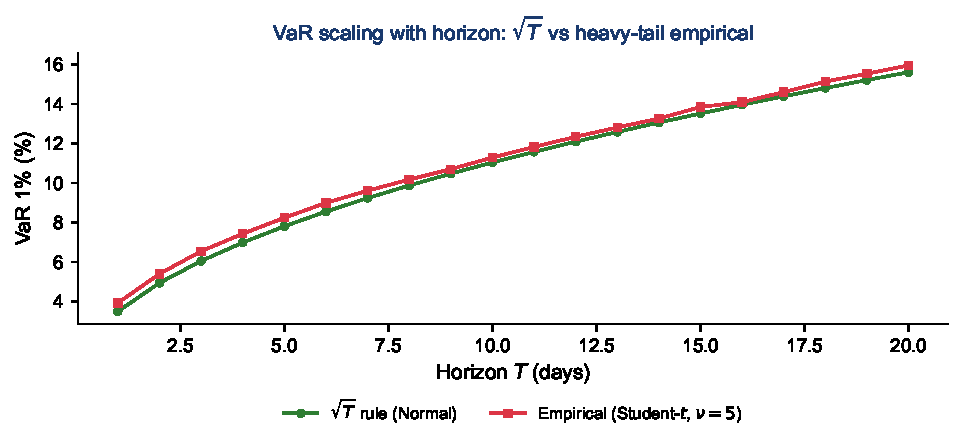
\includegraphics[width=\linewidth]{ch11_var_horizons.pdf}
    \end{center}
    {\scriptsize\textcolor{MediumGray}{\textit{Regula $\sqrt{T}$ vs.\ VaR empiric sub Student-$t_5$. Diferența crește cu orizontul.}}}
    \end{column}
    \begin{column}{0.43\textwidth}
    \begin{itemize}\setlength{\itemsep}{0pt}
        \item Sub i.i.d.\ Normal: $\VaR^{(T)} = \sqrt{T} \cdot \VaR^{(1)}$
        \item \textbf{Sub cozi grele}: regula \textbf{subestimează} (CLT lent)
        \item \textbf{Sub autocorelație pozitivă}:
        \[
        \Var(R_T) \approx T\sigma^2 \cdot \tfrac{1+\phi}{1-\phi}
        \]
        $\Rightarrow$ subestimare la $\phi > 0$
        \item Basel cere VaR 10 zile; în practică se aplică $\sqrt{10}$ pe VaR 1 zi
        \item \textbf{Diebold et al.\ (1997)}: \textit{,,square-root rule is dangerous''}
    \end{itemize}
    \end{column}
    \end{columns}
    \quantlet{SFM\_ch11\_var\_horizons}{https://github.com/danpele/SFM/tree/main/Quantlets/Ch_11/SFM_ch11_var_horizons}
    \end{cminipage}
\end{frame}

\begin{frame}[shrink=10]{Eșecul subaditivității VaR (Embrechts)}
    \begin{cminipage}{0.95\textwidth}
    \begin{columns}[T]
    \begin{column}{0.55\textwidth}
    \begin{center}
    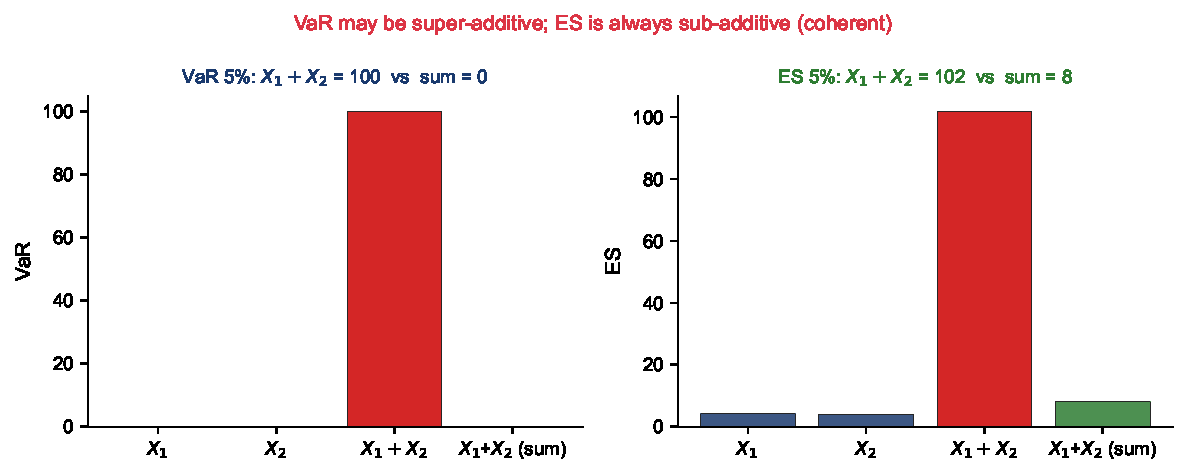
\includegraphics[width=\linewidth]{ch11_subadditivity.pdf}
    \end{center}
    {\scriptsize\textcolor{MediumGray}{\textit{VaR-ul portofoliului depășește suma VaR-urilor individuale (failure). ES respectă subaditivitatea.}}}
    \end{column}
    \begin{column}{0.43\textwidth}
    \begin{itemize}\setlength{\itemsep}{0pt}
        \item \textbf{Subaditivitate (A2)}: $\rho(X+Y) \leq \rho(X) + \rho(Y)$
        \item \textbf{Contraexemplu}: 2 obligațiuni cu default rar, $\Pr = 4\%$, pierdere 100 EUR
        \item Individual: $\VaR_{5\%} = 0$ (4\% $<$ 5\%)
        \item Portofoliu: $\Pr(\geq 1 \text{ default}) = 7{,}84\%$ $\Rightarrow$ $\VaR_{5\%} = 100$
        \item $100 > 0 + 0$ \textbf{\textcolor{Crimson}{(eșec subaditivitate)}}
        \item ES nu suferă $\Rightarrow$ motivul tranziției FRTB
    \end{itemize}
    \end{column}
    \end{columns}
    \quantlet{SFM\_ch11\_subadditivity}{https://github.com/danpele/SFM/tree/main/Quantlets/Ch_11/SFM_ch11_subadditivity}
    \end{cminipage}
\end{frame}

\begin{frame}[shrink=10]{Date de lucru: privire de ansamblu}
\begin{columns}[T,onlytextwidth]
    \begin{column}{0.58\textwidth}
    \begin{center}
    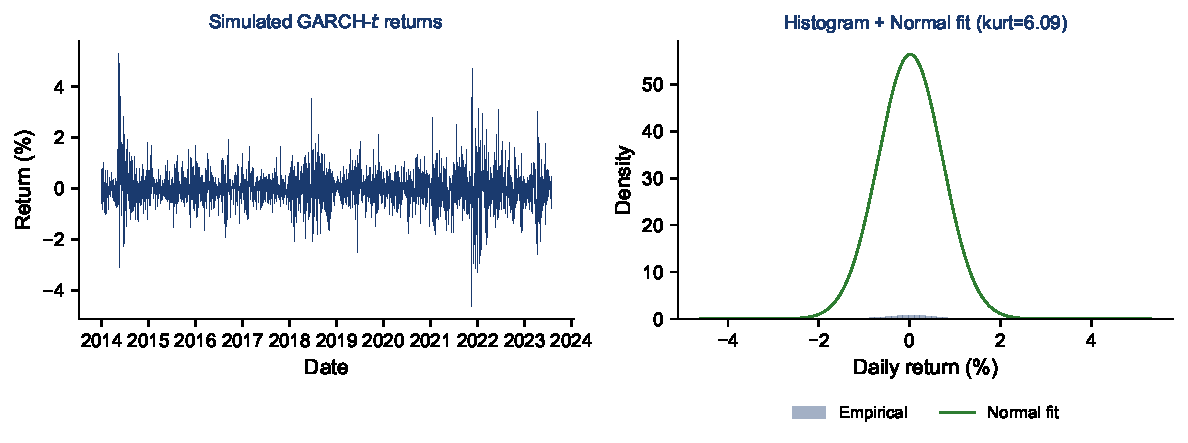
\includegraphics[width=\linewidth]{ch11_returns_overview.pdf}
    \end{center}
    \end{column}
    \begin{column}{0.40\textwidth}
    \begin{block}{Setul simulat}
    \begin{itemize}\setlength{\itemsep}{0pt}
        \item 2500 randamente zilnice GARCH(1,1)-$t_6$ simulate
        \item $\sigma_{\mathrm{anualizat}} \approx 11\%$; skewness $\approx -0{,}2$; kurtoză $\approx 6$
    \end{itemize}
    \end{block}
    \begin{exampleblock}{De ce simulat?}
    \begin{itemize}\setlength{\itemsep}{0pt}
        \item Replicabilitate: \texttt{np.random.seed(42)}
        \item Avem \emph{adevărul} pentru backtesting
        \item Comparabil cu acțiuni reale (BVB, SPY)
    \end{itemize}
    \end{exampleblock}
    \end{column}
\end{columns}
\quantlet{SFM\_ch11\_returns\_overview}{https://github.com/danpele/SFM/tree/main/Quantlets/Ch_11/SFM_ch11_returns_overview}
\end{frame}

\begin{frame}[shrink=10]{Monte Carlo VaR --- paths și histograme P\&L}
\begin{columns}[T,onlytextwidth]
    \begin{column}{0.58\textwidth}
    \begin{center}
    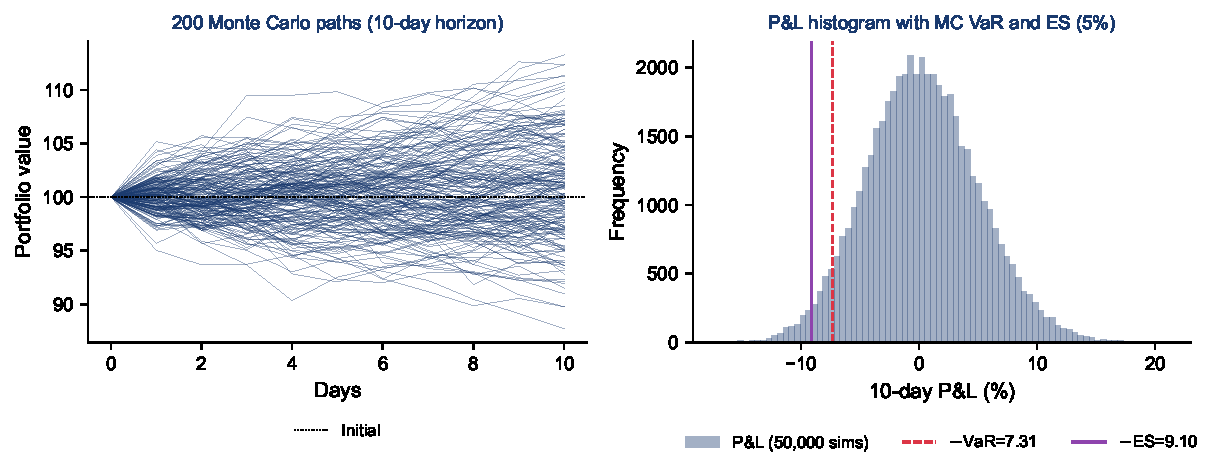
\includegraphics[width=\linewidth]{ch11_method_mc.pdf}
    \end{center}
    \end{column}
    \begin{column}{0.40\textwidth}
    \begin{block}{Algoritm MC pentru VaR}
    \begin{itemize}\setlength{\itemsep}{0pt}
        \item Simulează $M = 50\,000$ traiectorii GBM pe $h = 10$ zile
        \item Calculează P\&L final $L_m = V_0(S_m(h)/S_0 - 1)$
        \item $\widehat{\VaR}_\alpha = -Q_\alpha(\{L_m\})$
    \end{itemize}
    \end{block}
    \begin{alertblock}{Considerente}
    \begin{itemize}\setlength{\itemsep}{0pt}
        \item Eroare $\propto 1/\sqrt{M}$; pentru $\alpha = 0{,}1\%$ nevoie $M \geq 10^6$
        \item Variance reduction: antithetic, control variates
        \item Quasi-MC (Sobol): convergență $\sim 1/M$ în dimensiuni joase
    \end{itemize}
    \end{alertblock}
    \end{column}
\end{columns}
\quantlet{SFM\_ch11\_method\_mc}{https://github.com/danpele/SFM/tree/main/Quantlets/Ch_11/SFM_ch11_method_mc}
\end{frame}

%=============================================================================
% TEHNICI AVANSATE (VIZUALIZĂRI)
%=============================================================================
\section{Tehnici Avansate de VaR}

\begin{frame}[shrink=10]{Cornish-Fisher --- corecție pentru asimetrie și cozi}
\begin{columns}[T,onlytextwidth]
    \begin{column}{0.58\textwidth}
    \begin{center}
    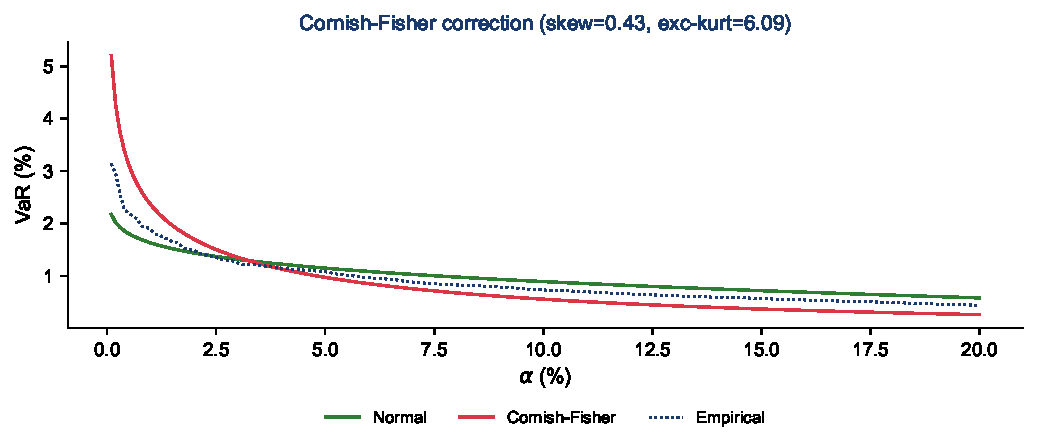
\includegraphics[width=\linewidth]{ch11_cornish_fisher.pdf}
    \end{center}
    \end{column}
    \begin{column}{0.40\textwidth}
    \begin{block}{Expansiunea CF}
    \begin{align*}
    z^{CF}_\alpha &= z + \tfrac{z^2-1}{6}s + \tfrac{z^3-3z}{24}k\\
    & \quad - \tfrac{2z^3-5z}{36}s^2
    \end{align*}
    \end{block}
    \begin{alertblock}{Lecție}
    \begin{itemize}\setlength{\itemsep}{0pt}
        \item Corecție de \emph{moment}; nu schimbă forma distribuției
        \item Skew $<0$ + kurtoză $\Rightarrow$ \textbf{crește} VaR cu 30--60\%
        \item Limita: $|s|\leq 1$, $k \leq 6$
    \end{itemize}
    \end{alertblock}
    \end{column}
\end{columns}
\quantlet{SFM\_ch11\_cornish\_fisher}{https://github.com/danpele/SFM/tree/main/Quantlets/Ch_11/SFM_ch11_cornish_fisher}
\end{frame}

\begin{frame}[shrink=10]{Filtered Historical Simulation (Hull-White 1998)}
\begin{columns}[T,onlytextwidth]
    \begin{column}{0.58\textwidth}
    \begin{center}
    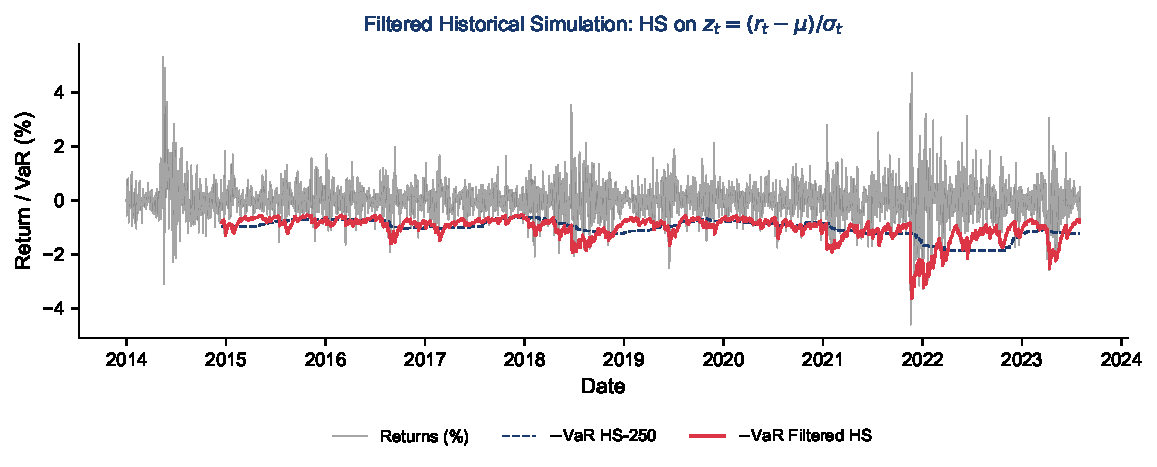
\includegraphics[width=\linewidth]{ch11_filtered_hs.pdf}
    \end{center}
    \end{column}
    \begin{column}{0.40\textwidth}
    \begin{block}{Algoritm FHS}
    \begin{enumerate}\setlength{\itemsep}{0pt}
        \item Fit GARCH(1,1); calculează $\hat{\sigma}_t$
        \item Standardizează: $\hat{z}_t = r_t/\hat{\sigma}_t$
        \item $\VaR^{FHS}_{t+1} = -\hat{\sigma}_{t+1} \cdot Q_\alpha(\hat{z})$
    \end{enumerate}
    \end{block}
    \begin{alertblock}{Avantaj}
    \begin{itemize}\setlength{\itemsep}{0pt}
        \item Combină \emph{reactivitate} GARCH cu \emph{forma empirică} a cozii
        \item Mai bun ca HS și GARCH-Normal în Basel 2011
    \end{itemize}
    \end{alertblock}
    \end{column}
\end{columns}
\quantlet{SFM\_ch11\_filtered\_hs}{https://github.com/danpele/SFM/tree/main/Quantlets/Ch_11/SFM_ch11_filtered_hs}
\end{frame}

\begin{frame}[shrink=10]{GJR-GARCH --- efectul de levier (asimetrie volatilitate)}
\begin{columns}[T,onlytextwidth]
    \begin{column}{0.58\textwidth}
    \begin{center}
    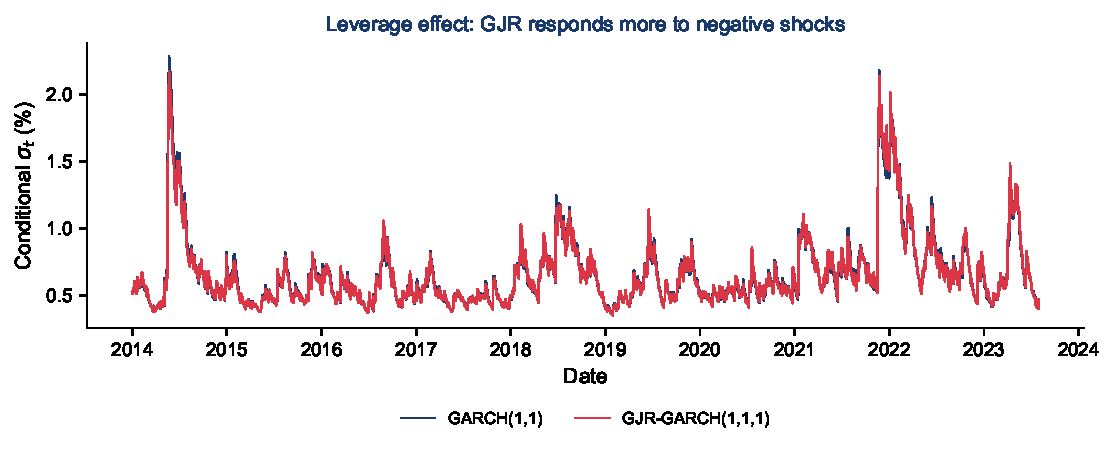
\includegraphics[width=\linewidth]{ch11_gjr_garch.pdf}
    \end{center}
    \end{column}
    \begin{column}{0.40\textwidth}
    \begin{block}{Modelul GJR (Glosten et al. 1993)}
    $$\sigma^2_t = \omega + (\alpha + \gamma I_{t-1}) r^2_{t-1} + \beta\sigma^2_{t-1}$$
    cu $I_{t-1} = \mathbf{1}\{r_{t-1} < 0\}$.
    \end{block}
    \begin{alertblock}{Implicație VaR}
    \begin{itemize}\setlength{\itemsep}{0pt}
        \item Black (1976): firma scade $\Rightarrow$ leverage $\uparrow$ $\Rightarrow$ vol $\uparrow$
        \item GARCH simetric subestimează $\sigma_{t+1}$ după zile negative
        \item Alternative: EGARCH, APARCH, TGARCH
    \end{itemize}
    \end{alertblock}
    \end{column}
\end{columns}
\quantlet{SFM\_ch11\_gjr\_garch}{https://github.com/danpele/SFM/tree/main/Quantlets/Ch_11/SFM_ch11_gjr_garch}
\end{frame}

\begin{frame}[shrink=10]{Hill plot --- estimarea indicelui cozii}
\begin{columns}[T,onlytextwidth]
    \begin{column}{0.58\textwidth}
    \begin{center}
    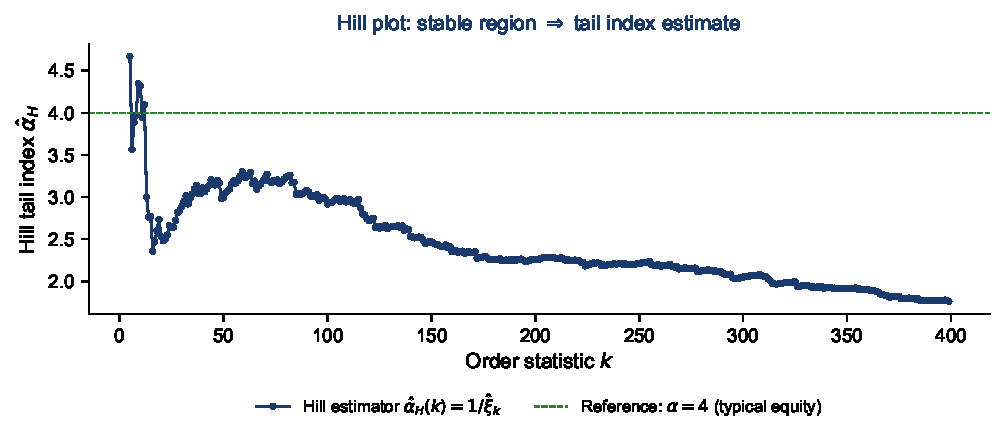
\includegraphics[width=\linewidth]{ch11_hill_plot.pdf}
    \end{center}
    \end{column}
    \begin{column}{0.40\textwidth}
    \begin{block}{Hill estimator}
    $$\hat{\xi}_H(k) = \tfrac{1}{k}\sum_{i=1}^k \ln(X_{(i)}/X_{(k+1)})$$
    cu $X_{(1)} \geq X_{(2)} \geq \dots$ ordonate.
    \end{block}
    \begin{alertblock}{Citire grafic}
    \begin{itemize}\setlength{\itemsep}{0pt}
        \item Căutați \textbf{platoul de stabilitate} ($k$ în care $\hat{\xi}_H$ se stabilizează)
        \item Indicele cozii $\alpha = 1/\hat{\xi}_H$; momentele $\mathbb{E}[L^p]$ finite doar pentru $p < \alpha$
        \item Equități tipic $\xi \in [0{,}2, 0{,}4]$
    \end{itemize}
    \end{alertblock}
    \end{column}
\end{columns}
\quantlet{SFM\_ch11\_hill\_plot}{https://github.com/danpele/SFM/tree/main/Quantlets/Ch_11/SFM_ch11_hill_plot}
\end{frame}

\begin{frame}[shrink=10]{Block Maxima --- GEV pe maxime lunare}
\begin{columns}[T,onlytextwidth]
    \begin{column}{0.58\textwidth}
    \begin{center}
    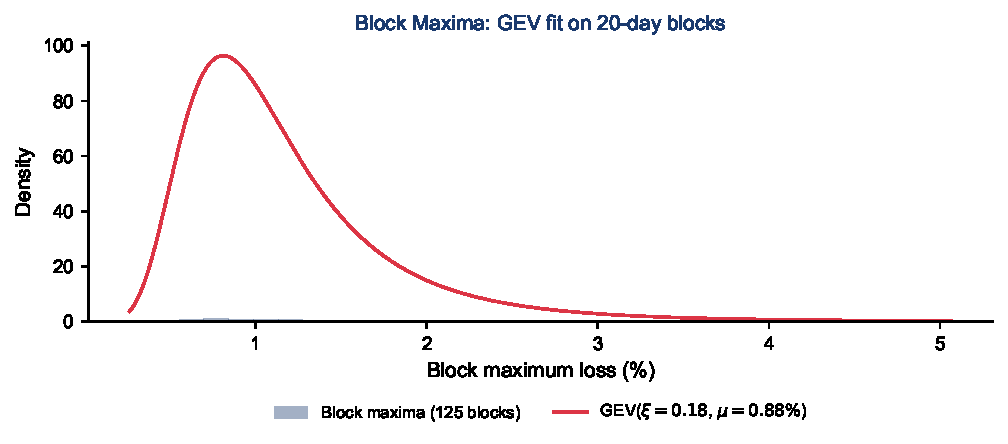
\includegraphics[width=\linewidth]{ch11_block_maxima.pdf}
    \end{center}
    \end{column}
    \begin{column}{0.40\textwidth}
    \begin{block}{GEV (Fisher-Tippett)}
    Maximele de blocuri converg la $\mathrm{GEV}(\mu, \sigma, \xi)$:
    \begin{itemize}\setlength{\itemsep}{0pt}
        \item $\xi > 0$: Fréchet (cozi grele)
        \item $\xi = 0$: Gumbel (exponential decay)
        \item $\xi < 0$: Weibull (mărginit superior)
    \end{itemize}
    \end{block}
    \begin{alertblock}{Return level $T$-an}
    $$z_T = \mu + \tfrac{\sigma}{\xi}\!\left[(-\ln(1-1/T))^{-\xi} - 1\right]$$
    Reglator: ,,o-dată-pe-100-ani'' eveniment
    \end{alertblock}
    \end{column}
\end{columns}
\quantlet{SFM\_ch11\_block\_maxima}{https://github.com/danpele/SFM/tree/main/Quantlets/Ch_11/SFM_ch11_block_maxima}
\end{frame}

\begin{frame}[shrink=10]{Lopez loss --- ranking modele VaR}
\begin{columns}[T,onlytextwidth]
    \begin{column}{0.58\textwidth}
    \begin{center}
    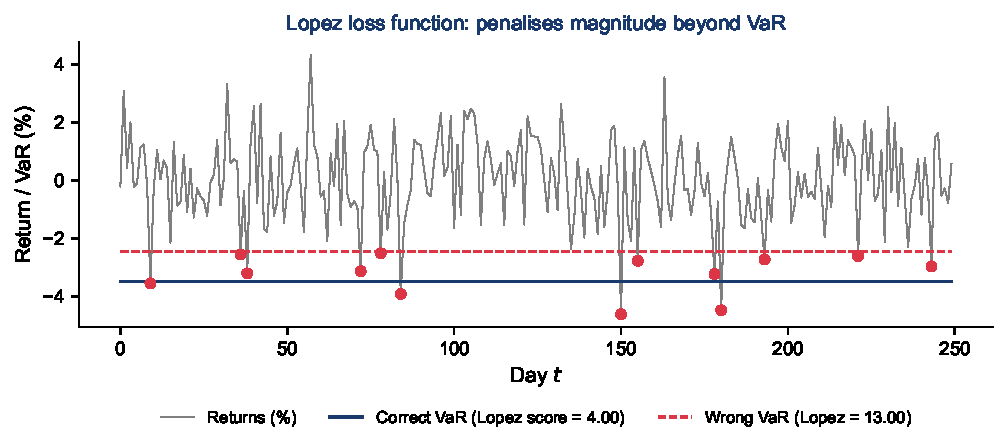
\includegraphics[width=\linewidth]{ch11_lopez_loss.pdf}
    \end{center}
    \end{column}
    \begin{column}{0.40\textwidth}
    \begin{block}{Funcția Lopez (1998)}
    $$L_t = \begin{cases} 1 + (r_t + \VaR_t)^2 & I_t = 1\\ 0 & I_t = 0\end{cases}$$
    Penalizează \emph{număr} + \emph{magnitudine}.
    \end{block}
    \begin{alertblock}{Folosire}
    \begin{itemize}\setlength{\itemsep}{0pt}
        \item \textbf{Ranking model selection}: model cu $\sum L_t$ minim preferat
        \item Nu este test statistic formal (fără $p$-value)
        \item Alternativ: Blanco-Ihle (continuă)
        \item Pentru ES: Acerbi-Szekely $Z$-tests
    \end{itemize}
    \end{alertblock}
    \end{column}
\end{columns}
\quantlet{SFM\_ch11\_lopez\_loss}{https://github.com/danpele/SFM/tree/main/Quantlets/Ch_11/SFM_ch11_lopez_loss}
\end{frame}

\begin{frame}[shrink=10]{LVaR --- VaR ajustat pentru lichiditate (Bangia et al.)}
\begin{columns}[T,onlytextwidth]
    \begin{column}{0.58\textwidth}
    \begin{center}
    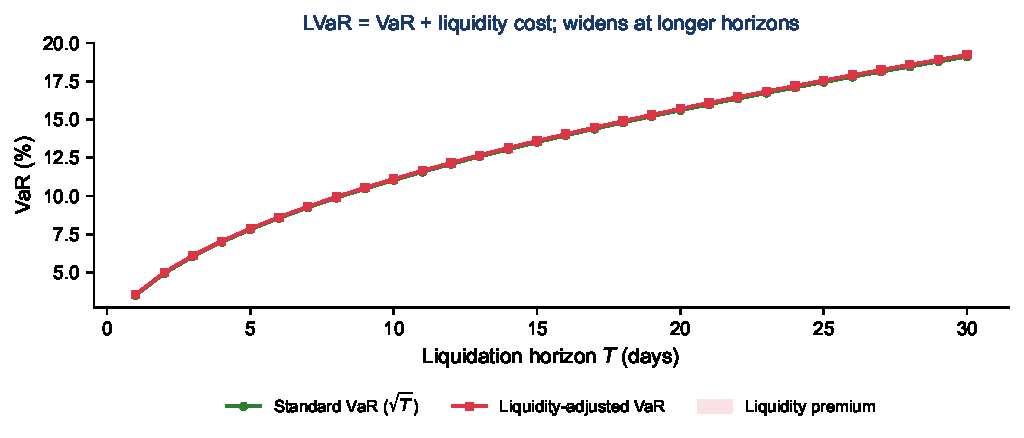
\includegraphics[width=\linewidth]{ch11_lvar.pdf}
    \end{center}
    \end{column}
    \begin{column}{0.40\textwidth}
    \begin{block}{Formula LVaR}
    $$\mathrm{LVaR} = \VaR + \tfrac{V}{2}(\mu_s + k\sigma_s)$$
    cu $\mu_s$ spread mediu, $\sigma_s$ vol spread, $k = z_{1-\alpha}$.
    \end{block}
    \begin{alertblock}{Impact}
    \begin{itemize}\setlength{\itemsep}{0pt}
        \item Pentru active iliquide: $\mathrm{LVaR}$ poate \textbf{dubla} VaR clasic
        \item Basel FRTB: \textbf{liquidity horizons} 10/20/40/60/120 zile pe asset class
        \item LTCM (1998): a ignorat costul lichidării forțate
    \end{itemize}
    \end{alertblock}
    \end{column}
\end{columns}
\quantlet{SFM\_ch11\_lvar}{https://github.com/danpele/SFM/tree/main/Quantlets/Ch_11/SFM_ch11_lvar}
\end{frame}

\begin{frame}[shrink=10]{Distribuția numărului de depășiri (binomial 250 zile)}
\begin{columns}[T,onlytextwidth]
    \begin{column}{0.58\textwidth}
    \begin{center}
    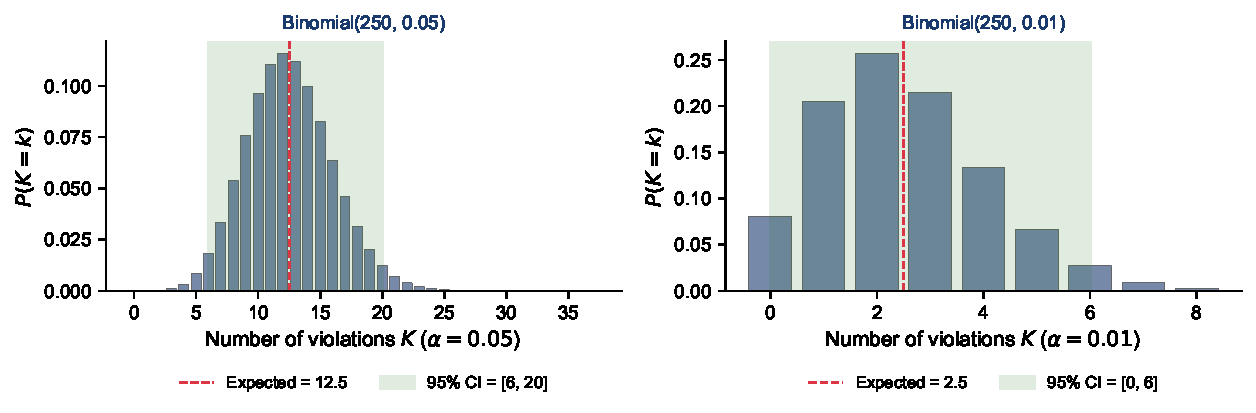
\includegraphics[width=\linewidth]{ch11_violation_dist.pdf}
    \end{center}
    \end{column}
    \begin{column}{0.40\textwidth}
    \begin{block}{Distribuție așteptată}
    Sub $H_0$: $K \sim \mathrm{Bin}(n, \alpha)$
    \begin{itemize}\setlength{\itemsep}{0pt}
        \item $\alpha = 1\%$, $n=250$: $\mathbb{E}[K] = 2{,}5$
        \item $\alpha = 5\%$, $n=250$: $\mathbb{E}[K] = 12{,}5$
        \item $\alpha = 0{,}1\%$, $n=250$: $\mathbb{E}[K] = 0{,}25$
    \end{itemize}
    \end{block}
    \begin{alertblock}{Citire CI 95\%}
    \begin{itemize}\setlength{\itemsep}{0pt}
        \item Interval Clopper-Pearson sau Wilson
        \item Basel zone trafic: bazate pe percentile sub $H_0$
        \item Putere statistică \textbf{joasă} pentru $\alpha$ mic
    \end{itemize}
    \end{alertblock}
    \end{column}
\end{columns}
\quantlet{SFM\_ch11\_violation\_dist}{https://github.com/danpele/SFM/tree/main/Quantlets/Ch_11/SFM_ch11_violation_dist}
\end{frame}

%=============================================================================
% TEST GRILĂ
%=============================================================================
\section{Test Grilă}

\begin{frame}[shrink=10]{Test 1: Definiția VaR}
\begin{cminipage}{0.95\textwidth}
    \begin{alertblock}{Întrebare}
    Care este definiția corectă a $\VaR_{1\%}$ pentru un portofoliu?
    \end{alertblock}
    \vspace{0.4cm}
    \begin{block}{Variante de răspuns}
    \textcolor{MainBlue}{\textbf{(A)}} Pierderea medie zilnică \\[3pt]
    \textcolor{MainBlue}{\textbf{(B)}} Pierderea maximă care nu este depășită cu probabilitate 99\% \\[3pt]
    \textcolor{MainBlue}{\textbf{(C)}} Pierderea care apare în 1\% din cele mai bune zile \\[3pt]
    \textcolor{MainBlue}{\textbf{(D)}} Volatilitatea zilnică înmulțită cu $\sqrt{252}$
    \end{block}
\end{cminipage}
\end{frame}

\begin{frame}[shrink=10]{Test 1: Răspuns}
\begin{cminipage}{0.95\textwidth}
    \begin{exampleblock}{Răspuns: B}
    $\VaR_{1\%}$ este pierderea care nu va fi depășită cu probabilitate 99\%; echivalent, este depășită cu probabilitate 1\%.
    \end{exampleblock}
    \vspace{0.2cm}
    \begin{itemize}\setlength{\itemsep}{0pt}
        \item \textbf{Explicație:}
        \item Formal: $\VaR_\alpha = \inf\{\ell : \Pr(L > \ell) \leq \alpha\} = -F_X^{-1}(\alpha)$
        \item \textbf{(A)} este incorect --- media pierderii este $\E[L]$, nu o cuantilă
        \item \textbf{(C)} este invers --- VaR privește \textbf{cele mai rele} zile, nu cele mai bune
        \item \textbf{(D)} este regula $\sqrt{T}$ pentru anualizare, nu VaR
        \item \textbf{Atenție convenție}: $\VaR_\alpha > 0$ reprezintă o \textbf{mărime de pierdere}
    \end{itemize}
\end{cminipage}
\end{frame}

\begin{frame}[shrink=10]{Test 2: VaR Normal pe portofoliu de 1M EUR}
\begin{cminipage}{0.95\textwidth}
    \begin{alertblock}{Întrebare}
    Portofoliu $V = 1.000.000$ EUR, $\mu = 0$, $\sigma = 1{,}5\%$ zilnic.
    Sub ipoteza de normalitate, cât este $\VaR_{1\%}$ zilnic?
    ($z_{0{,}01} = -2{,}326$)
    \end{alertblock}
    \vspace{0.4cm}
    \begin{block}{Variante de răspuns}
    \textcolor{MainBlue}{\textbf{(A)}} 15.000 EUR \\[3pt]
    \textcolor{MainBlue}{\textbf{(B)}} 24.675 EUR \\[3pt]
    \textcolor{MainBlue}{\textbf{(C)}} 34.890 EUR \\[3pt]
    \textcolor{MainBlue}{\textbf{(D)}} 46.350 EUR
    \end{block}
\end{cminipage}
\end{frame}

\begin{frame}[shrink=10]{Test 2: Răspuns}
\begin{cminipage}{0.95\textwidth}
    \begin{exampleblock}{Răspuns: C}
    $\VaR_{1\%} = V \cdot \sigma \cdot |z_{0{,}01}| = 1.000.000 \times 0{,}015 \times 2{,}326 = \mathbf{34.890}$ EUR.
    \end{exampleblock}
    \vspace{0.2cm}
    \begin{itemize}\setlength{\itemsep}{0pt}
        \item \textbf{Explicație:}
        \item Formulă: $\VaR_\alpha = -V \cdot (\mu + \sigma z_\alpha)$; cu $\mu = 0$ devine $V \sigma |z_\alpha|$
        \item \textbf{(B)} este $\VaR_{5\%}$ ($1{,}645 \times 1\% \times V \times 1{,}5$): nivel mai puțin sever
        \item \textbf{(D)} este $\VaR_{0{,}1\%}$ ($z = -3{,}090$): nivel extrem
        \item \textbf{Interpretare}: cu probabilitate 99\%, pierderea zilnică nu depășește 34.890 EUR
        \item \textbf{Echivalent}: așteptăm $\approx 2{,}5$ depășiri pe an (250 zile $\times$ 1\%)
        \item \textbf{Scalare 10 zile (Basel)}: $34.890 \times \sqrt{10} = 110.327$ EUR
    \end{itemize}
    \quantlet{SFM\_ch11\_method\_normal}{https://github.com/danpele/SFM/tree/main/Quantlets/Ch_11/SFM_ch11_method_normal}
\end{cminipage}
\end{frame}

\begin{frame}[shrink=10]{Test 3: VaR și subaditivitatea}
\begin{cminipage}{0.95\textwidth}
    \begin{alertblock}{Întrebare}
    Care dintre următoarele afirmații despre VaR este \textbf{adevărată}?
    \end{alertblock}
    \vspace{0.4cm}
    \begin{block}{Variante de răspuns}
    \textcolor{MainBlue}{\textbf{(A)}} VaR este întotdeauna subaditiv: diversificarea reduce VaR-ul total \\[3pt]
    \textcolor{MainBlue}{\textbf{(B)}} VaR este coerent și satisface toate axiomele Artzner et al.\ (1999) \\[3pt]
    \textcolor{MainBlue}{\textbf{(C)}} VaR poate eșua subaditivitatea pe distribuții non-eliptice (e.g., default discret) \\[3pt]
    \textcolor{MainBlue}{\textbf{(D)}} VaR și ES sunt echivalente sub Normală
    \end{block}
\end{cminipage}
\end{frame}

\begin{frame}[shrink=10]{Test 3: Răspuns}
\begin{cminipage}{0.95\textwidth}
    \begin{exampleblock}{Răspuns: C}
    VaR poate eșua subaditivitatea pe distribuții non-eliptice --- contraexemplul clasic Embrechts cu obligațiuni cu default rar.
    \end{exampleblock}
    \vspace{0.2cm}
    \begin{itemize}\setlength{\itemsep}{0pt}
        \item \textbf{Explicație:}
        \item \textbf{Contraexemplu}: 2 obligațiuni cu $\Pr(\text{default}) = 4\%$, pierdere 100 EUR fiecare
        \item Individual: $\VaR_{5\%} = 0$ (4\% $<$ 5\%)
        \item Portofoliu: $\Pr(\text{cel puțin un default}) = 7{,}84\%$ $\Rightarrow$ $\VaR_{5\%} = 100 > 0+0$
        \item \textbf{(A), (B)} sunt false --- exact motivul pentru care FRTB a trecut la ES
        \item \textbf{(D)} este fals --- chiar sub Normală, $\ES_{5\%} = 2{,}06\sigma > \VaR_{5\%} = 1{,}64\sigma$
        \item \textbf{ES este coerentă} (Acerbi--Tasche 2002) $\Rightarrow$ înlocuiește VaR sub FRTB
    \end{itemize}
\end{cminipage}
\end{frame}

\begin{frame}[shrink=10]{Test 4: Compararea metodelor pe cozi grele}
\begin{cminipage}{0.95\textwidth}
    \begin{alertblock}{Întrebare}
    Date cu cozi grele, $\nu = 5$. La ce nivel $\alpha$ \textbf{diferența} dintre $\VaR^{t}$ și $\VaR^{N}$ este \textbf{cea mai mare} ca raport?
    \end{alertblock}
    \vspace{0.4cm}
    \begin{block}{Variante de răspuns}
    \textcolor{MainBlue}{\textbf{(A)}} $\alpha = 10\%$ \\[3pt]
    \textcolor{MainBlue}{\textbf{(B)}} $\alpha = 5\%$ \\[3pt]
    \textcolor{MainBlue}{\textbf{(C)}} $\alpha = 1\%$ \\[3pt]
    \textcolor{MainBlue}{\textbf{(D)}} $\alpha = 0{,}1\%$
    \end{block}
\end{cminipage}
\end{frame}

\begin{frame}[shrink=10]{Test 4: Răspuns}
\begin{cminipage}{0.95\textwidth}
    \begin{exampleblock}{Răspuns: D}
    La $\alpha = 0{,}1\%$, raportul $\VaR^{t_5}/\VaR^{N} \approx 1{,}65$ --- cea mai mare diferență.
    \end{exampleblock}
    \vspace{0.2cm}
    \begin{itemize}\setlength{\itemsep}{0pt}
        \item \textbf{Explicație:}
        \item Sub Normală, cuantilele scad rapid pe coadă (densitate $\propto e^{-z^2/2}$)
        \item Sub Student-$t_5$, scad polinomial $\propto z^{-(\nu+1)} = z^{-6}$ --- mult mai lent
        \item \textbf{Regula degetului}: la $\alpha = 1\%$, $\VaR^{t_5} \approx 1{,}25 \times \VaR^{N}$
        \item La $\alpha = 0{,}1\%$, $\VaR^{t_5} \approx 1{,}65 \times \VaR^{N}$
        \item \textbf{Capital regulator}: ipoteza Normală subestimează capitalul cu 60--80\% la cuantile extreme
        \item \textbf{Lecția 1998 (LTCM)}: ,,4 SD o-dată-la-mileniu'' s-au repetat în 6 luni
    \end{itemize}
\end{cminipage}
\end{frame}

\begin{frame}[shrink=10]{Test 5: Backtesting Kupiec}
\begin{cminipage}{0.95\textwidth}
    \begin{alertblock}{Întrebare}
    Pentru un model VaR cu $n = 250$ zile și $\alpha = 5\%$, observăm $x = 18$ depășiri.
    Care este concluzia testului Kupiec POF la prag de semnificație 5\%? ($\chi^2_1(0{,}95) = 3{,}84$)
    \end{alertblock}
    \vspace{0.4cm}
    \begin{block}{Variante de răspuns}
    \textcolor{MainBlue}{\textbf{(A)}} Respingem $H_0$: modelul subestimează VaR-ul \\[3pt]
    \textcolor{MainBlue}{\textbf{(B)}} Respingem $H_0$: modelul supraestimează VaR-ul \\[3pt]
    \textcolor{MainBlue}{\textbf{(C)}} Nu respingem $H_0$: model acceptabil \\[3pt]
    \textcolor{MainBlue}{\textbf{(D)}} Testul nu se poate aplica deoarece $x > n\alpha$
    \end{block}
\end{cminipage}
\end{frame}

\begin{frame}[shrink=10]{Test 5: Răspuns}
\begin{cminipage}{0.95\textwidth}
    \begin{exampleblock}{Răspuns: C}
    $LR_{POF} = 2{,}43 < 3{,}84$ $\Rightarrow$ nu respingem $H_0$. Modelul este acceptabil.
    \end{exampleblock}
    \vspace{0.2cm}
    \begin{itemize}\setlength{\itemsep}{0pt}
        \item \textbf{Explicație:}
        \item Depășiri așteptate: $n\alpha = 12{,}5$; observate: $x = 18$; $\hat{p} = 0{,}072$
        \item $LR_{POF} = -2\ln\!\left[\frac{0{,}05^{18}\, 0{,}95^{232}}{0{,}072^{18}\, 0{,}928^{232}}\right] \approx 2{,}43$
        \item $p$-value $\approx 0{,}119 > 0{,}05$ $\Rightarrow$ nu respingem $H_0$
        \item \textbf{Intuitiv}: 18 e mai mult decât așteptat (12{,}5), dar într-un interval de încredere binomial rezonabil
        \item \textbf{Atenție}: Kupiec testează doar (P1) acoperirea necondițională; depășirile pot fi totuși \textbf{clusterizate}
        \item \textbf{Pentru clustering}: aplicăm Christoffersen IC sau Engle--Manganelli DQ
    \end{itemize}
\end{cminipage}
\end{frame}

\begin{frame}[shrink=10]{Test 6: Basel Traffic Light}
\begin{cminipage}{0.95\textwidth}
    \begin{alertblock}{Întrebare}
    Un model VaR 99\% pe $n = 250$ zile produce $K = 7$ depășiri. În ce zonă Basel se află și care este capitalul de risc de piață?
    \end{alertblock}
    \vspace{0.4cm}
    \begin{block}{Variante de răspuns}
    \textcolor{MainBlue}{\textbf{(A)}} Verde, $m = 3{,}00$ \\[3pt]
    \textcolor{MainBlue}{\textbf{(B)}} Galben, $m = 3{,}65$ \\[3pt]
    \textcolor{MainBlue}{\textbf{(C)}} Roșu, $m = 4{,}00$ \\[3pt]
    \textcolor{MainBlue}{\textbf{(D)}} Verde, $m = 2{,}50$
    \end{block}
\end{cminipage}
\end{frame}

\begin{frame}[shrink=10]{Test 6: Răspuns}
\begin{cminipage}{0.95\textwidth}
    \begin{exampleblock}{Răspuns: B}
    $K = 7 \in [5, 9]$ $\Rightarrow$ zona \textcolor{Amber}{galben}, add-on $\approx 0{,}65$; multiplier $m = 3{,}65$.
    \end{exampleblock}
    \vspace{0.2cm}
    \begin{itemize}\setlength{\itemsep}{0pt}
        \item \textbf{Explicație:}
        \item Verde: $0$--$4$ depășiri, $m = 3{,}00$ (probabilitate sub $H_0$: 89{,}2\%)
        \item Galben: $5$--$9$ depășiri, $m = 3{,}40$--$3{,}85$ (probabilitate sub $H_0$: 10{,}8\%)
        \item Roșu: $\geq 10$ depășiri, $m = 4{,}00$ (probabilitate sub $H_0$: 0{,}01\%)
        \item \textbf{Capital de risc de piață}: $\text{RC} = m \cdot \VaR^{10d}_{99\%}$
        \item \textbf{Implicație}: pierdere de 25\% din profit pentru bancă (3 $\to$ 3{,}65)
        \item \textbf{Penalizare asimetrică}: subestimarea (zona galbenă) costă, supraestimarea nu este penalizată
    \end{itemize}
    \quantlet{SFM\_ch11\_traffic\_light}{https://github.com/danpele/SFM/tree/main/Quantlets/Ch_11/SFM_ch11_traffic_light}
\end{cminipage}
\end{frame}

\begin{frame}[shrink=10]{Test 7: Scalarea pe orizont}
\begin{cminipage}{0.95\textwidth}
    \begin{alertblock}{Întrebare}
    Dacă $\VaR^{1d}_{1\%} = 1.000$ EUR și aplicăm regula $\sqrt{T}$, cât este $\VaR^{10d}_{1\%}$ aproximativ? Când e \textbf{problematică} această regulă?
    \end{alertblock}
    \vspace{0.4cm}
    \begin{block}{Variante de răspuns}
    \textcolor{MainBlue}{\textbf{(A)}} 10.000 EUR; e problematică sub i.i.d. Normal \\[3pt]
    \textcolor{MainBlue}{\textbf{(B)}} 3.162 EUR; e exactă sub orice distribuție \\[3pt]
    \textcolor{MainBlue}{\textbf{(C)}} 3.162 EUR; subestimează la cozi grele sau autocorelație pozitivă \\[3pt]
    \textcolor{MainBlue}{\textbf{(D)}} 1.000 EUR; VaR-ul nu scalează cu orizontul
    \end{block}
\end{cminipage}
\end{frame}

\begin{frame}[shrink=10]{Test 7: Răspuns}
\begin{cminipage}{0.95\textwidth}
    \begin{exampleblock}{Răspuns: C}
    $\VaR^{10d} = \sqrt{10} \cdot \VaR^{1d} = 3{,}162 \cdot 1.000 = \mathbf{3.162}$ EUR; subestimează la cozi grele sau autocorelație pozitivă.
    \end{exampleblock}
    \vspace{0.2cm}
    \begin{itemize}\setlength{\itemsep}{0pt}
        \item \textbf{Explicație:}
        \item Regula $\sqrt{T}$ derivă din $\Var(R_{1:T}) = T \sigma^2$ sub i.i.d.\ Normal
        \item \textbf{Sub cozi grele}: $\VaR^{(T)} > \sqrt{T} \VaR^{(1)}$ (CLT lent pe cozi)
        \item \textbf{Sub autocorelație pozitivă}: $\Var(R_{1:T}) \approx T \sigma^2 \cdot \frac{1+\phi}{1-\phi}$ $\Rightarrow$ subestimare
        \item \textbf{Diebold et al.\ (1997)}: ,,square-root rule is dangerous''
        \item \textbf{Basel cere VaR 10 zile} --- în practică se aplică $\sqrt{10}$, dar instituțiile mari prognozează direct la 10 zile
        \item \textbf{(A)} confundă scalarea cu liniaritate; \textbf{(B)} ignoră ipotezele
    \end{itemize}
\end{cminipage}
\end{frame}

\begin{frame}[shrink=10]{Test 8: VaR vs ES sub FRTB}
\begin{cminipage}{0.95\textwidth}
    \begin{alertblock}{Întrebare}
    De ce regulatorul (BCBS) a trecut prin FRTB (2016+) de la \textbf{VaR 99\%} la \textbf{ES 97{,}5\%}?
    \end{alertblock}
    \vspace{0.4cm}
    \begin{block}{Variante de răspuns}
    \textcolor{MainBlue}{\textbf{(A)}} ES e mai ușor de calculat decât VaR \\[3pt]
    \textcolor{MainBlue}{\textbf{(B)}} ES e coerentă (subaditivă) și surprinde severitatea pierderilor extreme \\[3pt]
    \textcolor{MainBlue}{\textbf{(C)}} ES dă un capital mai mic, favorabil băncilor \\[3pt]
    \textcolor{MainBlue}{\textbf{(D)}} VaR 99\% este interzis în UE
    \end{block}
\end{cminipage}
\end{frame}

\begin{frame}[shrink=10]{Test 8: Răspuns}
\begin{cminipage}{0.95\textwidth}
    \begin{exampleblock}{Răspuns: B}
    ES este coerentă (subaditivă) și surprinde \textbf{severitatea} pierderilor extreme --- exact ce VaR nu poate.
    \end{exampleblock}
    \vspace{0.2cm}
    \begin{itemize}\setlength{\itemsep}{0pt}
        \item \textbf{Explicație:}
        \item Sub Normală: $\ES_{97{,}5\%} \approx \VaR_{99\%}$ (calibrare echivalentă)
        \item Sub cozi grele: $\ES_{97{,}5\%} > \VaR_{99\%}$ $\Rightarrow$ capital mai mare pentru active riscante
        \item \textbf{(A)} este fals --- ES e mai dificil (backtesting în special)
        \item \textbf{(C)} este fals --- pe cozi grele ES dă capital \textbf{mai mare}, nu mai mic
        \item \textbf{(D)} este fals --- VaR rămâne folosit pentru calibrare și raportare internă
        \item \textbf{Backtesting ES}: nu este \textit{elicitable} (problema Gneiting 2011); se folosesc teste Acerbi--Szekely
    \end{itemize}
    \quantlet{SFM\_ch11\_es\_var\_ratio}{https://github.com/danpele/SFM/tree/main/Quantlets/Ch_11/SFM_ch11_es_var_ratio}
\end{cminipage}
\end{frame}

\begin{frame}[shrink=10]{Test 9: Cornish-Fisher pentru randamente asimetrice}
    \begin{cminipage}{0.95\textwidth}
    \begin{alertblock}{Întrebare}
    Cu $z = -2{,}326$, $s = -0{,}5$, $k = 2$, care este \emph{semnul} corecției Cornish-Fisher principale pentru $\VaR_{1\%}$?
    \end{alertblock}
    \begin{block}{Variante de răspuns}
    \begin{itemize}\setlength{\itemsep}{0pt}
        \item \textbf{(A)} Pozitivă (scade $\VaR$ în valoare absolută)
        \item \textbf{(B)} Negativă (crește $\VaR$ în valoare absolută)
        \item \textbf{(C)} Zero --- expansiunea nu se aplică
        \item \textbf{(D)} Depinde doar de $k$, nu de $s$
    \end{itemize}
    \end{block}
    \end{cminipage}
\end{frame}

\begin{frame}[shrink=10]{Test 9: Răspuns}
    \begin{cminipage}{0.95\textwidth}
    \begin{exampleblock}{Răspuns: B}
    Skewness $< 0$ + kurtoză excesivă $\Rightarrow$ termenii $\frac{z^2-1}{6}s < 0$ și $\frac{z^3-3z}{24}k < 0$ scad $z^{CF}$, mărind $\VaR$ în valoare absolută cu $\sim 40$--$60\%$.
    \end{exampleblock}
    \begin{itemize}\setlength{\itemsep}{0pt}
        \item \textbf{Explicație:} $z^{CF} = z + \frac{z^2-1}{6}s + \frac{z^3-3z}{24}k - \frac{2z^3-5z}{36}s^2$
        \item \textbf{Numeric:} $z^{CF} = -2{,}326 + 0{,}735(-0{,}5) + (-0{,}233)(2) - (-0{,}375)(0{,}25) = -3{,}066$
        \item Asimetria negativă (skew $<0$): pierderile extreme \emph{ascunse} sub Normal
        \item Limita modelului: $|s| \leq 1$, $k \leq 6$ pentru convergență
    \end{itemize}
    \quantlet{SFM\_ch11\_cornish\_fisher}{https://github.com/danpele/SFM/tree/main/Quantlets/Ch_11/SFM_ch11_cornish_fisher}
    \end{cminipage}
\end{frame}

\begin{frame}[shrink=10]{Test 10: GJR-GARCH și efectul de levier}
    \begin{cminipage}{0.95\textwidth}
    \begin{alertblock}{Întrebare}
    GJR-GARCH(1,1): $\sigma^2_t = \omega + \alpha r^2_{t-1} + \gamma r^2_{t-1}\mathbf{1}\{r_{t-1}<0\} + \beta\sigma^2_{t-1}$. Cu $\alpha = 0{,}03$, $\gamma = 0{,}12$, $\beta = 0{,}85$. Care este raportul impact șoc $-3\%$ vs $+3\%$?
    \end{alertblock}
    \begin{block}{Variante de răspuns}
    \begin{itemize}\setlength{\itemsep}{0pt}
        \item \textbf{(A)} $1{,}0$ (simetric)
        \item \textbf{(B)} $2{,}0$
        \item \textbf{(C)} $5{,}0$
        \item \textbf{(D)} $10{,}0$
    \end{itemize}
    \end{block}
    \end{cminipage}
\end{frame}

\begin{frame}[shrink=10]{Test 10: Răspuns}
    \begin{cminipage}{0.95\textwidth}
    \begin{exampleblock}{Răspuns: C}
    Raport = $(\alpha + \gamma)/\alpha = (0{,}03 + 0{,}12)/0{,}03 = \mathbf{5{,}0}$. Șocurile negative ridică volatilitatea de 5 ori mai mult decât cele pozitive.
    \end{exampleblock}
    \begin{itemize}\setlength{\itemsep}{0pt}
        \item \textbf{Leverage effect (Black 1976)}: firma scade $\Rightarrow$ debt/equity $\uparrow$ $\Rightarrow$ vol $\uparrow$
        \item Persistența: $\alpha + \gamma/2 + \beta = 0{,}94 < 1$ (stationar)
        \item GARCH simetric subestimează $\sigma_{t+1}$ după zile negative $\Rightarrow$ depășiri VaR clusterizate
        \item Alternative: \textbf{EGARCH} (Nelson 1991), \textbf{APARCH}, \textbf{TGARCH}
    \end{itemize}
    \quantlet{SFM\_ch11\_gjr\_garch}{https://github.com/danpele/SFM/tree/main/Quantlets/Ch_11/SFM_ch11_gjr_garch}
    \end{cminipage}
\end{frame}

\begin{frame}[shrink=10]{Test 11: Hill estimator și indicele cozii}
    \begin{cminipage}{0.95\textwidth}
    \begin{alertblock}{Întrebare}
    Hill estimator dă $\hat{\xi}_H = 0{,}40$. Ce momente $\mathbb{E}[L^p]$ ale pierderii sunt \textbf{garantat finite}?
    \end{alertblock}
    \begin{block}{Variante de răspuns}
    \begin{itemize}\setlength{\itemsep}{0pt}
        \item \textbf{(A)} Toate ($p$ orice valoare)
        \item \textbf{(B)} $p < 1/0{,}40 = 2{,}5$ (varianța nu există)
        \item \textbf{(C)} $p \leq 2$ (doar media și varianța)
        \item \textbf{(D)} Niciun moment finit
    \end{itemize}
    \end{block}
    \end{cminipage}
\end{frame}

\begin{frame}[shrink=10]{Test 11: Răspuns}
    \begin{cminipage}{0.95\textwidth}
    \begin{exampleblock}{Răspuns: B}
    Indicele cozii $\alpha = 1/\hat{\xi}_H = 2{,}5$. Momentele $\mathbb{E}[L^p]$ există doar pentru $p < \alpha$ = 2{,}5. \textbf{Varianța nu există} ($p=2$ marginal); kurtoză (p=4) și skewness (p=3) absent.
    \end{exampleblock}
    \begin{itemize}\setlength{\itemsep}{0pt}
        \item Teorie Karamata: $\Pr(L > x) \sim x^{-\alpha}\ell(x)$ cu $\ell$ slowly varying
        \item Implicație: \textbf{LLN funcționează}, dar \textbf{CLT nu} pentru $\alpha < 2$ (stable laws)
        \item Active cu $\xi \approx 0{,}5$ (FX emergente, crypto): nu se aplică Sharpe ratio, $z$-score VaR Normal
        \item Diebold-Schuermann-Stroughair (2000): folosiți EVT, nu Normal, pentru $\alpha < 4$
    \end{itemize}
    \quantlet{SFM\_ch11\_hill\_plot}{https://github.com/danpele/SFM/tree/main/Quantlets/Ch_11/SFM_ch11_hill_plot}
    \end{cminipage}
\end{frame}

\begin{frame}[shrink=10]{Test 12: Liquidity-adjusted VaR (LVaR)}
    \begin{cminipage}{0.95\textwidth}
    \begin{alertblock}{Întrebare}
    LVaR (Bangia et al. 1999) adaugă o ajustare la $\VaR$ pentru bid-ask spread. Formula simplă: $\mathrm{LVaR} = \VaR + \frac{1}{2}V \cdot \mu_s$ unde $\mu_s$ = spread mediu. Pentru poziție $V = 1$M EUR, spread $= 30$ bps, $\VaR_{1\%} = 25\,000$ EUR, care este $\mathrm{LVaR}$?
    \end{alertblock}
    \begin{block}{Variante de răspuns}
    \begin{itemize}\setlength{\itemsep}{0pt}
        \item \textbf{(A)} $25\,000$ EUR (spread irelevant)
        \item \textbf{(B)} $26\,500$ EUR
        \item \textbf{(C)} $40\,000$ EUR
        \item \textbf{(D)} $55\,000$ EUR
    \end{itemize}
    \end{block}
    \end{cminipage}
\end{frame}

\begin{frame}[shrink=10]{Test 12: Răspuns}
    \begin{cminipage}{0.95\textwidth}
    \begin{exampleblock}{Răspuns: B}
    $\mathrm{LVaR} = 25\,000 + 0{,}5 \cdot 1\,000\,000 \cdot 0{,}003 = 25\,000 + 1\,500 = \mathbf{26\,500}$ EUR (\textit{+6\%}).
    \end{exampleblock}
    \begin{itemize}\setlength{\itemsep}{0pt}
        \item Costul lichidității crește cu \textbf{varianța spread-ului} ($\sigma_s$): formulă completă $\frac{V}{2}(\mu_s + k \sigma_s)$
        \item Pentru active iliquide (real estate, private equity): LVaR poate \textbf{dubla} VaR clasic
        \item Basel FRTB introduce \textbf{liquidity horizons} diferențiate (10, 20, 40, 60, 120 zile)
        \item LTCM (1998) și Long-Term Volatility Fund: au \emph{ignorat} costul lichidării forțate
    \end{itemize}
    \quantlet{SFM\_ch11\_lvar}{https://github.com/danpele/SFM/tree/main/Quantlets/Ch_11/SFM_ch11_lvar}
    \end{cminipage}
\end{frame}

\begin{frame}[shrink=10]{Test 13: Lopez loss vs Kupiec POF}
    \begin{cminipage}{0.95\textwidth}
    \begin{alertblock}{Întrebare}
    Două modele VaR au aceeași frecvență de depășiri (12 în 250 zile), dar magnitudini diferite. Kupiec POF nu poate distinge. Ce alternativă folosiți?
    \end{alertblock}
    \begin{block}{Variante de răspuns}
    \begin{itemize}\setlength{\itemsep}{0pt}
        \item \textbf{(A)} Christoffersen IC (clustering)
        \item \textbf{(B)} \textbf{Lopez loss} (penalizează magnitudinea depășirilor)
        \item \textbf{(C)} Acerbi-Szekely (test pentru ES, nu VaR)
        \item \textbf{(D)} Niciun test --- frecvența egală e suficientă
    \end{itemize}
    \end{block}
    \end{cminipage}
\end{frame}

\begin{frame}[shrink=10]{Test 13: Răspuns}
    \begin{cminipage}{0.95\textwidth}
    \begin{exampleblock}{Răspuns: B}
    Lopez loss $L_t = (1 + (r_t + \VaR_t)^2)\mathbf{1}\{r_t < -\VaR_t\}$ penalizează atât \emph{numărul} cât și \emph{magnitudinea} depășirilor.
    \end{exampleblock}
    \begin{itemize}\setlength{\itemsep}{0pt}
        \item Kupiec testează doar $\hat{p} = x/n$ vs $\alpha$ --- ignoră dimensiunea depășirii
        \item Lopez: \textbf{loss function} pentru ranking model selection (nu test statistic formal)
        \item Util pentru raportare regulator: ,,câtă magnitudine media depășirile?''
        \item Alternativ: \textbf{Blanco-Ihle loss} (continuă vs Lopez discretă)
        \item Pentru ES specific: folosiți \textbf{Acerbi-Szekely Z-tests}
    \end{itemize}
    \quantlet{SFM\_ch11\_lopez\_loss}{https://github.com/danpele/SFM/tree/main/Quantlets/Ch_11/SFM_ch11_lopez_loss}
    \end{cminipage}
\end{frame}

\begin{frame}[shrink=10]{Test 14: Filtered HS vs HS clasic}
    \begin{cminipage}{0.95\textwidth}
    \begin{alertblock}{Întrebare}
    Filtered Historical Simulation (Hull-White 1998) combină GARCH cu HS. Care este \emph{avantajul} principal față de HS clasic?
    \end{alertblock}
    \begin{block}{Variante de răspuns}
    \begin{itemize}\setlength{\itemsep}{0pt}
        \item \textbf{(A)} Este parametric (asumă Normal)
        \item \textbf{(B)} Reactivează rapid la regimul curent de volatilitate, păstrând forma empirică a cozii
        \item \textbf{(C)} Calculează ES exact (nu doar VaR)
        \item \textbf{(D)} Nu necesită backtesting
    \end{itemize}
    \end{block}
    \end{cminipage}
\end{frame}

\begin{frame}[shrink=10]{Test 14: Răspuns}
    \begin{cminipage}{0.95\textwidth}
    \begin{exampleblock}{Răspuns: B}
    FHS reactivează rapid la regimul curent ($\hat{\sigma}_{t+1}$ de la GARCH) păstrând \emph{forma empirică} a cozii (cuantila pe $\hat{z}_t$, nu pe distribuție parametrică).
    \end{exampleblock}
    \begin{itemize}\setlength{\itemsep}{0pt}
        \item Formula: $\VaR^{FHS}_\alpha(t+1) = -\hat{\sigma}_{t+1} \cdot Q_\alpha(\{\hat{z}_s\}_{s \leq t})$
        \item HS clasic: \textbf{lent} la schimbarea regimului (fereastra 250 zile masquerade vol)
        \item GARCH parametric: rapid dar \textbf{asumă distribuție} (Normal, $t$); FHS evită asta
        \item Performanță superioară în Basel 2011 backtest exercise (Kuester et al. 2006)
        \item Costul: necesită convergența GARCH (probleme cu $\alpha + \beta \to 1$)
    \end{itemize}
    \quantlet{SFM\_ch11\_filtered\_hs}{https://github.com/danpele/SFM/tree/main/Quantlets/Ch_11/SFM_ch11_filtered_hs}
    \end{cminipage}
\end{frame}

%=============================================================================
% ADEVĂRAT / FALS
%=============================================================================
\section{Întrebări Adevărat/Fals}

\begin{frame}[shrink=10]{Adevărat/Fals --- partea I}
\begin{cminipage}{0.95\textwidth}
\begin{block}{Marcați A (adevărat) sau F (fals). Justificați}
\begin{enumerate}\setlength{\itemsep}{1pt}
    \item \textbf{[A/F]} $\VaR_{1\%}$ înseamnă o pierdere depășită cu probabilitate 99\%.
    \item \textbf{[A/F]} ES este întotdeauna mai mare sau egal cu VaR la același nivel $\alpha$.
    \item \textbf{[A/F]} Metoda HS necesită alegerea unei distribuții parametrice.
    \item \textbf{[A/F]} Sub ipoteza i.i.d.\ Normal, $\VaR$ scalează cu $\sqrt{T}$.
    \item \textbf{[A/F]} VaR este o măsură coerentă de risc.
\end{enumerate}
\end{block}
\vspace{0.15cm}
\begin{exampleblock}{Răspunsuri și justificări (1--5)}
\begin{enumerate}\setlength{\itemsep}{0pt}
    \item \textcolor{Crimson}{\textbf{F}} --- $\VaR_{1\%}$ este pierderea depășită cu probabilitate \textbf{1\%}, nu 99\%.
    \item \textcolor{Forest}{\textbf{A}} --- $\ES_\alpha$ este media valorilor în coada peste $\VaR_\alpha$ $\Rightarrow$ $\ES_\alpha \geq \VaR_\alpha$.
    \item \textcolor{Crimson}{\textbf{F}} --- HS este \textbf{non-parametrică}: folosește cuantila empirică a randamentelor observate.
    \item \textcolor{Forest}{\textbf{A}} --- doar sub i.i.d.\ Normal; cu cozi grele sau autocorelație, regula subestimează.
    \item \textcolor{Crimson}{\textbf{F}} --- VaR \textbf{eșuează} axioma de subaditivitate (A2) pe distribuții non-eliptice.
\end{enumerate}
\end{exampleblock}
\end{cminipage}
\end{frame}

\begin{frame}[shrink=10]{Adevărat/Fals --- partea II}
\begin{cminipage}{0.95\textwidth}
\begin{block}{Marcați A (adevărat) sau F (fals). Justificați}
\begin{enumerate}\setlength{\itemsep}{1pt}\setcounter{enumi}{5}
    \item \textbf{[A/F]} Sub VaR Normal, capital $\VaR_{1\%}$ subestimează riscul real al unei acțiuni cu $\nu = 4$.
    \item \textbf{[A/F]} Testul Kupiec POF detectează clustering-ul depășirilor VaR.
    \item \textbf{[A/F]} Zona galbenă Basel apare în $\approx 10{,}8\%$ din cazuri sub un model corect.
    \item \textbf{[A/F]} Metoda Monte Carlo are eroare $\propto 1/M$ unde $M$ e numărul de simulări.
    \item \textbf{[A/F]} ES este \textit{elicitable} și poate fi backtest-uit direct cu un \textit{scoring rule} strict consistent.
\end{enumerate}
\end{block}
\vspace{0.15cm}
\begin{exampleblock}{Răspunsuri și justificări (6--10)}
\begin{enumerate}\setlength{\itemsep}{0pt}\setcounter{enumi}{5}
    \item \textcolor{Forest}{\textbf{A}} --- cu $\nu = 4$, $\VaR^{t}_{1\%} \approx 1{,}3 \times \VaR^{N}_{1\%}$ $\Rightarrow$ Normalul subestimează capitalul.
    \item \textcolor{Crimson}{\textbf{F}} --- Kupiec testează doar (P1) acoperirea necondițională; pentru clustering folosim Christoffersen IC.
    \item \textcolor{Forest}{\textbf{A}} --- $\Pr(5 \leq K \leq 9 \mid K \sim \text{Bin}(250, 0{,}01)) \approx 10{,}8\%$.
    \item \textcolor{Crimson}{\textbf{F}} --- eroarea MC este $\propto 1/\sqrt{M}$; pentru $1/M$ avem nevoie de Quasi-MC (Sobol).
    \item \textcolor{Crimson}{\textbf{F}} --- ES nu e elicitable (Gneiting 2011); se backtest-uiește indirect (Acerbi--Szekely, ES/VaR ratio).
\end{enumerate}
\end{exampleblock}
\end{cminipage}
\end{frame}

\begin{frame}[shrink=10]{Adevărat/Fals --- partea III (metode avansate)}
\begin{cminipage}{0.95\textwidth}
\begin{block}{Marcați A (adevărat) sau F (fals). Justificați.}
\begin{enumerate}\setlength{\itemsep}{0pt}
    \item[11.] \textbf{[A/F]} Cornish-Fisher este o expansiune polinomială care converge pentru orice $s$, $k$.
    \item[12.] \textbf{[A/F]} Filtered HS extrage cuantila empirică din inovații standardizate GARCH.
    \item[13.] \textbf{[A/F]} GJR-GARCH adaugă un termen $\gamma$ care reacționează doar la șocuri pozitive.
    \item[14.] \textbf{[A/F]} Hill estimator $\hat{\xi}_H$ este consistent indiferent de alegerea lui $k$.
    \item[15.] \textbf{[A/F]} Lopez loss este un test statistic formal cu distribuție $\chi^2$.
\end{enumerate}
\end{block}
\begin{exampleblock}{Răspunsuri și justificări (11--15)}
\begin{enumerate}\setlength{\itemsep}{0pt}
    \item[11.] \textbf{F} --- valabil doar pentru $|s| \leq 1$ și $k \leq 6$; dincolo diverge.
    \item[12.] \textbf{A} --- $\VaR^{FHS}_{t+1} = -\hat{\sigma}_{t+1} \cdot Q_\alpha(\hat{z}_t)$ (Hull-White 1998).
    \item[13.] \textbf{F} --- $\gamma$ reacționează la șocuri \textbf{negative}: $\mathbf{1}\{r_{t-1} < 0\}$ (leverage effect).
    \item[14.] \textbf{F} --- $k$ mic $\Rightarrow$ varianță mare; $k$ mare $\Rightarrow$ bias; cere Hill plot pentru alegere.
    \item[15.] \textbf{F} --- este o \emph{loss function} pentru ranking, nu test cu distribuție; nu există $p$-value.
\end{enumerate}
\end{exampleblock}
\end{cminipage}
\end{frame}

%=============================================================================
% EXERCIȚII DE CALCUL
%=============================================================================
\section{Exerciții de Calcul}

\begin{frame}[shrink=10]{Exercițiul 1: VaR și ES Normal pe portofoliu}
    \begin{cminipage}{0.95\textwidth}
    \begin{block}{Enunț}
    \begin{itemize}\setlength{\itemsep}{0pt}
        \item Portofoliu $V = 500.000$ EUR, randament zilnic $r \sim \mathcal{N}(\mu, \sigma^2)$ cu $\mu = 0{,}05\%$, $\sigma = 1{,}2\%$.
        \item Calculați $\VaR$ și $\ES$ la $\alpha \in \{5\%, 1\%, 0{,}1\%\}$ pe orizont de 1 zi.
        \item $\phi(z_{0{,}05}) = 0{,}1031$, $\phi(z_{0{,}01}) = 0{,}0267$, $\phi(z_{0{,}001}) = 0{,}00337$
    \end{itemize}
    \end{block}
    \vspace{0.1cm}
    \begin{exampleblock}{Rezolvare}
    \begin{itemize}\setlength{\itemsep}{0pt}
        \item Formule: $\VaR_\alpha = -V(\mu + \sigma z_\alpha)$, \quad $\ES_\alpha = V(-\mu + \sigma \phi(z_\alpha)/\alpha)$
        \item $\VaR_{5\%} = -500.000(0{,}0005 - 0{,}012 \cdot 1{,}645) = \mathbf{9.620}$ EUR; \quad $\ES_{5\%} = \mathbf{12.122}$ EUR
        \item $\VaR_{1\%} = -500.000(0{,}0005 - 0{,}012 \cdot 2{,}326) = \mathbf{13.706}$ EUR; \quad $\ES_{1\%} = \mathbf{15.770}$ EUR
        \item $\VaR_{0{,}1\%} = -500.000(0{,}0005 - 0{,}012 \cdot 3{,}090) = \mathbf{18.290}$ EUR; \quad $\ES_{0{,}1\%} = \mathbf{19.972}$ EUR
        \item Raport $\ES/\VaR$: $1{,}26$ (la 5\%), $1{,}15$ (la 1\%), $1{,}09$ (la 0{,}1\%) --- scade cu $\alpha$
    \end{itemize}
    \end{exampleblock}
    \quantlet{SFM\_ch11\_method\_normal}{https://github.com/danpele/SFM/tree/main/Quantlets/Ch_11/SFM_ch11_method_normal}
    \end{cminipage}
\end{frame}

\begin{frame}[shrink=10]{Exercițiul 2: VaR istoric (HS) pe 20 zile}
    \begin{cminipage}{0.95\textwidth}
    \begin{block}{Enunț}
    Avem 20 randamente zilnice (\%) sortate crescător:
    \begin{center}
    \footnotesize
    $-3{,}5;\; -2{,}8;\; -2{,}1;\; -1{,}8;\; -1{,}5;\; -1{,}1;\; -0{,}9;\; -0{,}6;\; -0{,}3;\; -0{,}1;$ \\
    $\phantom{-}0{,}2;\; \phantom{-}0{,}4;\; \phantom{-}0{,}7;\; \phantom{-}0{,}9;\; \phantom{-}1{,}1;\; \phantom{-}1{,}3;\; \phantom{-}1{,}6;\; \phantom{-}2{,}0;\; \phantom{-}2{,}4;\; \phantom{-}3{,}1$
    \end{center}
    Calculați $\widehat{\VaR}_{5\%}^{HS}$, $\widehat{\VaR}_{10\%}^{HS}$ și $\widehat{\ES}_{10\%}^{HS}$.
    \end{block}
    \vspace{0.1cm}
    \begin{exampleblock}{Rezolvare}
    \begin{itemize}\setlength{\itemsep}{0pt}
        \item $\alpha = 5\%$: index $= \lceil 0{,}05 \cdot 20\rceil = 1$ $\Rightarrow$ $r_{(1)} = -3{,}5\%$ $\Rightarrow$ $\widehat{\VaR}_{5\%}^{HS} = \mathbf{3{,}5\%}$
        \item $\alpha = 10\%$: index $= \lceil 0{,}10 \cdot 20\rceil = 2$ $\Rightarrow$ $r_{(2)} = -2{,}8\%$ $\Rightarrow$ $\widehat{\VaR}_{10\%}^{HS} = \mathbf{2{,}8\%}$
        \item $\widehat{\ES}_{10\%}^{HS} = -\frac{1}{2}(r_{(1)} + r_{(2)}) = -\frac{1}{2}(-3{,}5 - 2{,}8) = \mathbf{3{,}15\%}$
    \end{itemize}
    \end{exampleblock}
    \begin{alertblock}{Atenție la fereastră}
    \begin{itemize}\setlength{\itemsep}{0pt}
        \item Cu $W = 20$, nu putem estima $\VaR_{1\%}$ (cuantila $0{,}2$ --- doar 1 observație disponibilă)
        \item Regulă: $\alpha \geq 2/W$ pentru estimare HS stabilă
    \end{itemize}
    \end{alertblock}
    \quantlet{SFM\_ch11\_method\_hs}{https://github.com/danpele/SFM/tree/main/Quantlets/Ch_11/SFM_ch11_method_hs}
    \end{cminipage}
\end{frame}

\begin{frame}[shrink=10]{Exercițiul 3: VaR Student-$t$ vs Normal}
    \begin{cminipage}{0.95\textwidth}
    \begin{block}{Enunț}
    Aceeași date: $\mu = 0$, $\sigma = 1\%$ zilnic. Comparați $\VaR_{1\%}$ Normal vs Student-$t_5$.
    \begin{itemize}\setlength{\itemsep}{0pt}
        \item $z_{0{,}01} = -2{,}326$ (Normal standard)
        \item $t_5^{-1}(0{,}01) = -3{,}365$ (Student-$t$ cu 5 gl)
    \end{itemize}
    \end{block}
    \vspace{0.1cm}
    \begin{exampleblock}{Rezolvare}
    \begin{itemize}\setlength{\itemsep}{0pt}
        \item Normal: $\VaR^{N}_{1\%} = -\sigma \cdot z_{0{,}01} = 1\% \cdot 2{,}326 = \mathbf{2{,}33\%}$
        \item Student-$t_5$ standardizat: cuantila ajustată $= \sqrt{(\nu-2)/\nu} \cdot t_5^{-1}(0{,}01) = \sqrt{3/5} \cdot (-3{,}365) = -2{,}607$
        \item $\VaR^{t_5}_{1\%} = -\sigma \cdot (-2{,}607) = 1\% \cdot 2{,}607 = \mathbf{2{,}61\%}$
        \item Raport: $\VaR^{t_5}_{1\%}/\VaR^{N}_{1\%} = 2{,}61/2{,}33 = \mathbf{1{,}12}$ --- creștere de 12\%
        \item La $\alpha = 0{,}1\%$: $t_5^{-1}(0{,}001) = -5{,}893$ $\Rightarrow$ $\VaR^{t_5}_{0{,}1\%} = 1\% \cdot 4{,}565 = 4{,}57\%$ vs $\VaR^{N}_{0{,}1\%} = 3{,}09\%$ --- creștere de 48\%
    \end{itemize}
    \end{exampleblock}
    \begin{alertblock}{Concluzie}
    \begin{itemize}\setlength{\itemsep}{0pt}
        \item Cu cât $\alpha$ mai mic, cu atât diferența crește $\Rightarrow$ Normalul subestimează \textbf{exact unde contează cel mai mult}
    \end{itemize}
    \end{alertblock}
    \quantlet{SFM\_ch11\_method\_student\_t}{https://github.com/danpele/SFM/tree/main/Quantlets/Ch_11/SFM_ch11_method_student_t}
    \end{cminipage}
\end{frame}

\begin{frame}[shrink=10]{Exercițiul 4: VaR pe portofoliu cu 2 active}
    \begin{cminipage}{0.95\textwidth}
    \begin{block}{Enunț}
    $V = 1.000.000$ EUR, $w_A = 0{,}6$, $w_B = 0{,}4$; $\sigma_A = 1{,}5\%$, $\sigma_B = 1\%$, $\rho_{AB} = 0{,}3$, $\mu = 0$.
    \begin{itemize}\setlength{\itemsep}{0pt}
        \item Calculați $\VaR_{1\%}^{port}$ sub Normala multivariată și comparați cu suma VaR-urilor individuale
    \end{itemize}
    \end{block}
    \begin{exampleblock}{Rezolvare}
    \begin{itemize}\setlength{\itemsep}{0pt}
        \item $\sigma_p^2 = w_A^2\sigma_A^2 + w_B^2\sigma_B^2 + 2w_A w_B \sigma_A \sigma_B \rho_{AB} = 1{,}186 \cdot 10^{-4}$ $\Rightarrow$ $\sigma_p = 1{,}089\%$
        \item $\VaR_{1\%}^{port} = V \sigma_p \cdot 2{,}326 = \mathbf{25.327}$ EUR
        \item Individual: $\VaR_A = 20.934$ EUR, $\VaR_B = 9.304$ EUR; suma $= 30.238$ EUR
        \item Portofoliu vs sumă: \textbf{economie 16{,}2\%} datorită diversificării
    \end{itemize}
    \end{exampleblock}
    \begin{alertblock}{Interpretare}
    \begin{itemize}\setlength{\itemsep}{0pt}
        \item Sub Normală, VaR este \textbf{subaditiv} $\Rightarrow$ diversificarea reduce VaR; garantat doar pe distribuții eliptice
    \end{itemize}
    \end{alertblock}
    \quantlet{SFM\_ch11\_cross\_asset}{https://github.com/danpele/SFM/tree/main/Quantlets/Ch_11/SFM_ch11_cross_asset}
    \end{cminipage}
\end{frame}

\begin{frame}[shrink=10]{Exercițiul 5: Backtesting Kupiec POF}
    \begin{cminipage}{0.95\textwidth}
    \begin{block}{Enunț}
    \begin{itemize}\setlength{\itemsep}{0pt}
        \item Model A: $n = 500$, $\alpha = 1\%$, observate $x = 12$ depășiri
        \item Model B: $n = 500$, $\alpha = 1\%$, observate $x = 3$ depășiri
        \item Aplicați testul Kupiec POF la prag de semnificație 5\%. Care model este acceptat?
    \end{itemize}
    \end{block}
    \vspace{0.1cm}
    \begin{exampleblock}{Rezolvare}
    \begin{itemize}\setlength{\itemsep}{0pt}
        \item Depășiri așteptate: $n\alpha = 5$
        \item \textbf{Model A}: $\hat{p}_A = 12/500 = 0{,}024$; $LR_{POF} = -2[12\ln(0{,}01/0{,}024) + 488\ln(0{,}99/0{,}976)] = \mathbf{8{,}21}$
        \item $p$-value $= \Pr(\chi^2_1 > 8{,}21) = 0{,}0042 < 0{,}05$ $\Rightarrow$ \textbf{respingem $H_0$}: model A \textcolor{Crimson}{subestimează} VaR-ul
        \item \textbf{Model B}: $\hat{p}_B = 3/500 = 0{,}006$; $LR_{POF} = -2[3\ln(0{,}01/0{,}006) + 497\ln(0{,}99/0{,}994)] = \mathbf{1{,}05}$
        \item $p$-value $= 0{,}305 > 0{,}05$ $\Rightarrow$ \textbf{nu respingem} $H_0$: model B este acceptat
    \end{itemize}
    \end{exampleblock}
    \begin{alertblock}{Atenție}
    \begin{itemize}\setlength{\itemsep}{0pt}
        \item Kupiec testează simetric; în practică, regulatorul penalizează \textbf{doar} subestimarea (Basel)
        \item Model A: 12 depășiri în loc de 5 $\Rightarrow$ zonă \textcolor{Crimson}{roșu} echivalent (capital mărit)
    \end{itemize}
    \end{alertblock}
    \quantlet{SFM\_ch11\_kupiec}{https://github.com/danpele/SFM/tree/main/Quantlets/Ch_11/SFM_ch11_kupiec}
    \end{cminipage}
\end{frame}

\begin{frame}[shrink=10]{Exercițiul 6: Christoffersen IC --- clustering}
    \begin{cminipage}{0.95\textwidth}
    \begin{block}{Enunț}
    Sequence-ul hit-uri pe 250 zile (1 = depășire) produce contoarele:
    \begin{center}
    \small
    $n_{00} = 220, \quad n_{01} = 5, \quad n_{10} = 5, \quad n_{11} = 5, \quad n = 235$
    \end{center}
    Calculați $LR_{IC}$ și interpretați.
    \end{block}
    \vspace{0.1cm}
    \begin{exampleblock}{Rezolvare}
    \begin{itemize}\setlength{\itemsep}{0pt}
        \item $\pi_{01} = 5/225 = 0{,}0222$;\, $\pi_{11} = 5/10 = 0{,}500$;\, $\pi_2 = 10/235 = 0{,}0426$
        \item $LR_{IC} = -2\ln\!\frac{(1-\pi_2)^{225}\pi_2^{10}}{(1-\pi_{01})^{220}\pi_{01}^{5}(1-\pi_{11})^{5}\pi_{11}^{5}} \approx \mathbf{12{,}5} > \chi^2_1(0{,}95) = 3{,}84$ $\Rightarrow$ \textbf{respingem} independența
    \end{itemize}
    \end{exampleblock}
    \begin{alertblock}{Interpretare}
    \begin{itemize}\setlength{\itemsep}{0pt}
        \item $\pi_{11} = 50\% \gg \pi_{01} = 2{,}2\%$ $\Rightarrow$ clustering tipic GARCH neacomodat
        \item \textbf{Soluție}: GARCH-VaR cu inovații Student-$t$
    \end{itemize}
    \end{alertblock}
    \quantlet{SFM\_ch11\_christoffersen}{https://github.com/danpele/SFM/tree/main/Quantlets/Ch_11/SFM_ch11_christoffersen}
    \end{cminipage}
\end{frame}

\begin{frame}[shrink=10]{Exercițiul 7: Non-subaditivitatea VaR (Embrechts)}
    \begin{cminipage}{0.95\textwidth}
    \begin{block}{Enunț}
    Două obligațiuni $X_1$, $X_2$ independente, default cu $\Pr = 4\%$ (pierdere 100 EUR), altfel 0.
    \begin{itemize}\setlength{\itemsep}{0pt}
        \item Calculați $\VaR_{5\%}(X_1)$, $\VaR_{5\%}(X_2)$ și $\VaR_{5\%}(X_1+X_2)$
        \item Arătați eșecul subaditivității
    \end{itemize}
    \end{block}
    \vspace{0.1cm}
    \begin{exampleblock}{Rezolvare}
    \begin{itemize}\setlength{\itemsep}{0pt}
        \item Individual: $\Pr(X_i > 0) = 4\% \leq 5\%$ $\Rightarrow$ $\VaR_{5\%}(X_i) = \mathbf{0}$
        \item Sumă: $\Pr(X_1{+}X_2 \geq 100) = 1 - 0{,}96^2 = 0{,}0784 > 5\%$;\, $\Pr(\geq 200) = 0{,}0016 \leq 5\%$ $\Rightarrow$ $\VaR_{5\%}(X_1{+}X_2) = \mathbf{100}$
        \item \textbf{Verificare}: $100 > 0 + 0$ $\Rightarrow$ \textcolor{Crimson}{\textbf{VaR eșuează subaditivitatea}}
    \end{itemize}
    \end{exampleblock}
    \begin{alertblock}{Lecție}
    \begin{itemize}\setlength{\itemsep}{0pt}
        \item Diversificarea \textbf{crește} VaR --- absurd; ES nu suferă $\Rightarrow$ motivul trecerii la ES sub FRTB
    \end{itemize}
    \end{alertblock}
    \quantlet{SFM\_ch11\_subadditivity}{https://github.com/danpele/SFM/tree/main/Quantlets/Ch_11/SFM_ch11_subadditivity}
    \end{cminipage}
\end{frame}

\begin{frame}[shrink=10]{Exercițiul 8: Basel Traffic Light și capital}
    \begin{cminipage}{0.95\textwidth}
    \begin{block}{Enunț}
    Banca raportează $\VaR^{10d}_{99\%} = 5.000.000$ EUR (medie pe ultimele 60 zile). Backtesting pe ultimele 250 zile: $K = 6$ depășiri.
    \begin{itemize}\setlength{\itemsep}{0pt}
        \item Determinați zona Basel și multiplier-ul
        \item Calculați capitalul de risc de piață (Market Risk Charge)
    \end{itemize}
    \end{block}
    \vspace{0.1cm}
    \begin{exampleblock}{Rezolvare}
    \begin{itemize}\setlength{\itemsep}{0pt}
        \item $K = 6 \in [5, 9]$ $\Rightarrow$ zona \textcolor{Amber}{\textbf{galben}}, add-on $\approx 0{,}50$; $m = 3{,}50$
        \item $\text{MRC} = m \cdot \VaR^{10d}_{99\%} = \mathbf{17.500.000}$ EUR (vs $15.000.000$ în zona verde)
        \item Cost al modelului mai puțin precis: \textbf{2{,}5 milioane EUR} capital imobilizat
    \end{itemize}
    \end{exampleblock}
    \begin{alertblock}{Practică}
    \begin{itemize}\setlength{\itemsep}{0pt}
        \item Basel III final (CRR3): \textbf{Stressed VaR} $\Rightarrow$ MRC $= m(\VaR + sVaR)$; FRTB înlocuiește VaR cu ES stresat + orizonturi diferențiate (10--120 zile)
    \end{itemize}
    \end{alertblock}
    \quantlet{SFM\_ch11\_traffic\_light}{https://github.com/danpele/SFM/tree/main/Quantlets/Ch_11/SFM_ch11_traffic_light}
    \end{cminipage}
\end{frame}

\begin{frame}[shrink=10]{Exercițiul 9: VaR EVT (POT) --- formula GPD}
    \begin{cminipage}{0.95\textwidth}
    \begin{block}{Enunț}
    Date: 1000 randamente; alegem prag $u = 2\%$ (pierdere); avem $N_u = 35$ excese.
    Estimare GPD prin MLE: $\hat{\xi} = 0{,}25$, $\hat{\sigma} = 0{,}008$.
    Calculați $\VaR^{POT}_{1\%}$ și $\ES^{POT}_{1\%}$.
    \end{block}
    \vspace{0.1cm}
    \begin{exampleblock}{Rezolvare}
    \begin{itemize}\setlength{\itemsep}{0pt}
        \item POT: $\VaR_\alpha = u + \frac{\hat{\sigma}}{\hat{\xi}}\!\left[\!\left(\frac{n}{N_u}\alpha\right)^{\!-\hat{\xi}} - 1\right]$; cu $n=1000$, $N_u=35$, $\alpha=0{,}01$: $\frac{n}{N_u}\alpha = 0{,}2857$
        \item $\VaR_{1\%}^{POT} = 0{,}02 + \frac{0{,}008}{0{,}25}\!\left[0{,}2857^{-0{,}25} - 1\right] = \mathbf{3{,}18\%}$
        \item $\ES_\alpha = \frac{\VaR_\alpha}{1-\hat{\xi}} + \frac{\hat{\sigma} - \hat{\xi}u}{1-\hat{\xi}}$ $\Rightarrow$ $\ES_{1\%}^{POT} = \mathbf{4{,}64\%}$
    \end{itemize}
    \end{exampleblock}
    \begin{alertblock}{Observație}
    \begin{itemize}\setlength{\itemsep}{0pt}
        \item $\hat{\xi} = 0{,}25 > 0$ $\Rightarrow$ cozi grele (moment $1/\xi = 4$); ES finit. Pentru $\alpha < N_u/n$, POT este robustă (HS epuizată)
    \end{itemize}
    \end{alertblock}
    \quantlet{SFM\_ch11\_evt\_var}{https://github.com/danpele/SFM/tree/main/Quantlets/Ch_11/SFM_ch11_evt_var}
    \end{cminipage}
\end{frame}

\begin{frame}[shrink=10]{Exercițiul 10: Capital sub VaR vs ES (FRTB)}
    \begin{cminipage}{0.95\textwidth}
    \begin{block}{Enunț}
    Portofoliu cu $\mu = 0$, $\sigma = 2\%$. Calculați:
    \begin{itemize}\setlength{\itemsep}{0pt}
        \item Sub Normală: $\VaR_{1\%}$ și $\ES_{2{,}5\%}$
        \item Sub Student-$t_4$: $\VaR_{1\%}$ și $\ES_{2{,}5\%}$
        \item Comentați tranziția Basel III $\to$ FRTB
    \end{itemize}
    Constante: $z_{0{,}01} = -2{,}326$, $\phi(z)/\alpha$ pentru $\alpha=2{,}5\%$ și Normală: $2{,}338$; pentru $t_4$, multiplicatori $\approx 1{,}3$ pe coadă.
    \end{block}
    \vspace{0.1cm}
    \begin{exampleblock}{Rezolvare}
    \begin{itemize}\setlength{\itemsep}{0pt}
        \item \textbf{Normal}: $\VaR^{N}_{1\%} = \mathbf{4{,}65\%}$, $\ES^{N}_{2{,}5\%} = \mathbf{4{,}68\%}$ (FRTB calibrat să producă același capital sub Normală)
        \item \textbf{Student-$t_4$}: $\sqrt{(\nu-2)/\nu}\,t_4^{-1}(0{,}01) = 2{,}649$ $\Rightarrow$ $\VaR^{t_4}_{1\%} = \mathbf{5{,}30\%}$ (+14\%); $\ES^{t_4}_{2{,}5\%} \approx \mathbf{6{,}20\%}$ (+33\%)
    \end{itemize}
    \end{exampleblock}
    \begin{alertblock}{Concluzie}
    \begin{itemize}\setlength{\itemsep}{0pt}
        \item Sub cozi grele: $\ES_{2{,}5\%} > \VaR_{1\%}$ $\Rightarrow$ \textbf{FRTB cere capital mai mare}; active cu cozi grele (emergente, crypto) penalizate mai sever
    \end{itemize}
    \end{alertblock}
    \quantlet{SFM\_ch11\_acerbi\_szekely}{https://github.com/danpele/SFM/tree/main/Quantlets/Ch_11/SFM_ch11_acerbi_szekely}
    \end{cminipage}
\end{frame}

\begin{frame}[shrink=10]{Exercițiul 11: Cornish-Fisher VaR cu skewness și kurtosis}
    \begin{cminipage}{0.95\textwidth}
    \begin{block}{Enunț}
    Randamente cu $\mu = 0$, $\sigma = 1{,}5\%$, $\hat{s} = -0{,}4$, $\hat{k} = 3{,}0$ (excess). Calculați $\VaR^{CF}_{1\%}$ și comparați cu $\VaR^N$.
    \end{block}
    \begin{exampleblock}{Rezolvare}
    \begin{itemize}\setlength{\itemsep}{0pt}
        \item $z = \Phi^{-1}(0{,}01) = -2{,}326$
        \item $z^{CF} = z + \frac{z^2-1}{6}s + \frac{z^3-3z}{24}k - \frac{2z^3-5z}{36}s^2$
        \item $= -2{,}326 + \frac{4{,}41}{6}(-0{,}4) + \frac{-5{,}6}{24}(3) - \frac{-13{,}5}{36}(0{,}16)$
        \item $= -2{,}326 - 0{,}294 - 0{,}700 + 0{,}060 = \mathbf{-3{,}260}$
        \item $\VaR^{CF}_{1\%} = 1{,}5\% \cdot 3{,}260 = \mathbf{4{,}89\%}$ vs $\VaR^N = 3{,}49\%$ (+40\%)
    \end{itemize}
    \end{exampleblock}
    \begin{alertblock}{Interpretare}
    \begin{itemize}\setlength{\itemsep}{0pt}
        \item Skewness negativă + kurtoză excesivă $\Rightarrow$ Cornish-Fisher \textbf{crește} VaR semnificativ
        \item Limita: valabil doar pentru $|s| \leq 1$, $k \leq 6$; dincolo, expansiunea diverge
    \end{itemize}
    \end{alertblock}
    \quantlet{SFM\_ch11\_cornish\_fisher}{https://github.com/danpele/SFM/tree/main/Quantlets/Ch_11/SFM_ch11_cornish_fisher}
    \end{cminipage}
\end{frame}

\begin{frame}[shrink=10]{Exercițiul 12: Block Maxima --- GEV pe maxime lunare}
    \begin{cminipage}{0.95\textwidth}
    \begin{block}{Enunț}
    Pe 10 ani date zilnice (120 luni) extragem maximul lunar al pierderilor. Fitting GEV produce: $\hat{\mu} = 2{,}1\%$, $\hat{\sigma} = 0{,}8\%$, $\hat{\xi} = 0{,}28$. Calculați $\VaR$ pentru perioada de retur de 1 an (252 zile).
    \end{block}
    \begin{exampleblock}{Rezolvare}
    \begin{itemize}\setlength{\itemsep}{0pt}
        \item $T$-year return level: $z_T = \mu + \frac{\sigma}{\xi}\!\left[\left(-\ln(1-1/T)\right)^{-\xi} - 1\right]$
        \item Pentru 252 zile = 12 luni $\Rightarrow$ $T = 12$ blocuri lunare
        \item $-\ln(1 - 1/12) = -\ln(0{,}9167) = 0{,}087$
        \item $z_{12} = 0{,}021 + \frac{0{,}008}{0{,}28}[0{,}087^{-0{,}28} - 1] = 0{,}021 + 0{,}0286 \cdot 0{,}811 = \mathbf{4{,}42\%}$
        \item $\hat{\xi} > 0$ $\Rightarrow$ Fréchet (cozi grele, polinomiale); pierderea maximă \textbf{nu este mărginită}
    \end{itemize}
    \end{exampleblock}
    \begin{alertblock}{Comparativ}
    \begin{itemize}\setlength{\itemsep}{0pt}
        \item Block Maxima: \emph{wasteful} (1 obs/lună), dar interpretabil regulator (,,o-dată-pe-an'')
        \item POT (excese peste prag): mai eficient statistic; folosit în Basel/Solvency II
    \end{itemize}
    \end{alertblock}
    \quantlet{SFM\_ch11\_block\_maxima}{https://github.com/danpele/SFM/tree/main/Quantlets/Ch_11/SFM_ch11_block_maxima}
    \end{cminipage}
\end{frame}

\begin{frame}[shrink=10]{Exercițiul 13: GJR-GARCH --- coeficient de levier}
    \begin{cminipage}{0.95\textwidth}
    \begin{block}{Enunț}
    Fit GJR-GARCH(1,1)-$t$ pe S\&P 500 produce: $\omega = 1{,}2\mathrm{e}{-6}$, $\alpha = 0{,}03$, $\gamma = 0{,}10$, $\beta = 0{,}88$. Comparați impactul unui șoc de $-3\%$ vs $+3\%$ asupra $\sigma^2_{t+1}$.
    \end{block}
    \begin{exampleblock}{Rezolvare}
    \begin{itemize}\setlength{\itemsep}{0pt}
        \item GJR: $\sigma^2_t = \omega + \alpha r^2_{t-1} + \gamma r^2_{t-1}\mathbf{1}\{r_{t-1}<0\} + \beta\sigma^2_{t-1}$
        \item Persistența: $\alpha + \gamma/2 + \beta = 0{,}03 + 0{,}05 + 0{,}88 = 0{,}96$ (aproape unit-root)
        \item Șoc $r_{t-1} = -3\%$: $\Delta \sigma^2 = (\alpha + \gamma)(0{,}03)^2 = 0{,}13 \cdot 9\mathrm{e}{-4} = 1{,}17\mathrm{e}{-4}$
        \item Șoc $r_{t-1} = +3\%$: $\Delta\sigma^2 = \alpha (0{,}03)^2 = 0{,}03 \cdot 9\mathrm{e}{-4} = 2{,}7\mathrm{e}{-5}$
        \item \textbf{Raport asimetrie}: $\frac{0{,}13}{0{,}03} = \mathbf{4{,}3\times}$ --- șocul negativ ridică volatilitatea de 4.3 ori mai mult
    \end{itemize}
    \end{exampleblock}
    \begin{alertblock}{Implicație VaR}
    \begin{itemize}\setlength{\itemsep}{0pt}
        \item GARCH simetric subestimează $\VaR_{t+1}$ după zile negative $\Rightarrow$ depășiri clusterizate
        \item GJR rezolvă ,,leverage effect'' (Black 1976): firma scade $\Rightarrow$ leverage $\uparrow$ $\Rightarrow$ vol $\uparrow$
    \end{itemize}
    \end{alertblock}
    \quantlet{SFM\_ch11\_gjr\_garch}{https://github.com/danpele/SFM/tree/main/Quantlets/Ch_11/SFM_ch11_gjr_garch}
    \end{cminipage}
\end{frame}

\begin{frame}[shrink=10]{Exercițiul 14: Hill estimator --- indicele cozii}
    \begin{cminipage}{0.95\textwidth}
    \begin{block}{Enunț}
    $n = 2500$ randamente; sortăm pierderile descendent: $X_{(1)} \geq X_{(2)} \geq \dots$. Pentru $k = 50$: $X_{(1)} = 0{,}095$, $X_{(50)} = 0{,}031$, $X_{(51)} = 0{,}030$. Suma $\sum_{i=1}^{50}\ln(X_{(i)}/X_{(51)}) = 14{,}25$.
    \end{block}
    \begin{exampleblock}{Rezolvare}
    \begin{itemize}\setlength{\itemsep}{0pt}
        \item $\hat{\xi}_H(k) = \frac{1}{k}\sum_{i=1}^{k}\ln(X_{(i)}/X_{(k+1)}) = 14{,}25/50 = \mathbf{0{,}285}$
        \item Indicele cozii $\alpha = 1/\hat{\xi}_H = 1/0{,}285 = \mathbf{3{,}51}$
        \item \textbf{Interpretare}: $\Pr(L > x) \sim C \cdot x^{-3{,}51}$ pentru $x$ mare $\Rightarrow$ cozi polinomiale
        \item Momentele $\mathbb{E}[L^p]$ există doar pentru $p < 3{,}51$ $\Rightarrow$ varianța există, kurtoză \emph{nu}
    \end{itemize}
    \end{exampleblock}
    \begin{alertblock}{Avertisment metodologic}
    \begin{itemize}\setlength{\itemsep}{0pt}
        \item Alegerea lui $k$ este critică: $k$ mic $\Rightarrow$ varianță mare; $k$ mare $\Rightarrow$ bias
        \item Soluție: \textbf{Hill plot} și căutați platou; alternativ moment estimator (Dekkers et al.)
    \end{itemize}
    \end{alertblock}
    \quantlet{SFM\_ch11\_hill\_plot}{https://github.com/danpele/SFM/tree/main/Quantlets/Ch_11/SFM_ch11_hill_plot}
    \end{cminipage}
\end{frame}

\begin{frame}[shrink=10]{Exercițiul 15: Lopez loss --- ranking modele VaR}
    \begin{cminipage}{0.95\textwidth}
    \begin{block}{Enunț}
    Două modele VaR, 250 zile, depășiri pe aceleași zile. Magnitudini: Model A $\{0{,}5\%, 1{,}2\%, 3{,}1\%\}$; Model B $\{0{,}3\%, 0{,}7\%, 2{,}0\%\}$. Calculați Lopez loss și ranguri.
    \end{block}
    \begin{exampleblock}{Rezolvare}
    \begin{itemize}\setlength{\itemsep}{0pt}
        \item $L_t = (1 + (r_t + \VaR_t)^2)\mathbf{1}\{r_t < -\VaR_t\}$ (pătratul depășirii)
        \item Model A: $L_A = (1+0{,}005^2) + (1+0{,}012^2) + (1+0{,}031^2) = 3 + 0{,}00104 = \mathbf{3{,}00104}$
        \item Model B: $L_B = (1+0{,}003^2) + (1+0{,}007^2) + (1+0{,}020^2) = 3 + 0{,}00058 = \mathbf{3{,}00058}$
        \item Ranking: \textbf{Model B preferat} (depășiri de aceeași frecvență dar magnitudine mai mică)
    \end{itemize}
    \end{exampleblock}
    \begin{alertblock}{De ce Lopez peste Kupiec?}
    \begin{itemize}\setlength{\itemsep}{0pt}
        \item Kupiec testează doar \emph{numărul} depășirilor; Lopez penalizează și \emph{magnitudinea}
        \item Util pentru \textbf{ranking model selection}; nu este test statistic formal
    \end{itemize}
    \end{alertblock}
    \quantlet{SFM\_ch11\_lopez\_loss}{https://github.com/danpele/SFM/tree/main/Quantlets/Ch_11/SFM_ch11_lopez_loss}
    \end{cminipage}
\end{frame}

%=============================================================================
% STUDII DE CAZ
%=============================================================================
\section{Studii de caz}

\begin{frame}[shrink=10]{Caz 1: Black Monday 1987 --- eșecul VaR Normal}
    \begin{cminipage}{0.95\textwidth}
    \begin{block}{Faptele}
    \begin{itemize}\setlength{\itemsep}{0pt}
        \item \textbf{19 octombrie 1987}: S\&P~500 scade $-22{,}6\%$ într-o singură zi
        \item Pe baza datelor 1980--1986: $\hat{\sigma} \approx 1\%$/zi, ipoteza Normalei părea rezonabilă
    \end{itemize}
    \end{block}
    \vspace{0.1cm}
    \begin{exampleblock}{Sub Normală cu $\mu = 0$, $\sigma = 1\%$}
    \begin{itemize}\setlength{\itemsep}{0pt}
        \item $z$-scor al evenimentului: $-22{,}6 / 1 = -22{,}6$
        \item Probabilitatea sub Normală: $\Pr(z \leq -22{,}6) \approx \mathbf{10^{-115}}$
        \item Echivalent: \textbf{un eveniment de o-dată-la-$10^{107}$ ani} (mai mult decât vârsta universului)
        \item $\VaR^{N}_{0{,}1\%} = 3{,}09\%$ vs.\ pierderea reală: $22{,}6\%$ --- subestimare \textbf{factor 7$\times$}
    \end{itemize}
    \end{exampleblock}
    \vspace{0.1cm}
    \begin{alertblock}{Sub Student-$t_4$ (cozi grele)}
    \begin{itemize}\setlength{\itemsep}{0pt}
        \item $\Pr(t_4 \leq -22{,}6) \approx 1{,}2 \cdot 10^{-5}$ --- de $10^{110}$ ori mai probabil
        \item Echivalent: \textbf{$\approx 1$ eveniment la 330 de ani} --- rar, dar plauzibil
        \item \textbf{Lecția 1987}: Normalele cu cozi subțiri nu pot prezice evenimente extreme; folosiți distribuții cu cozi grele
    \end{itemize}
    \end{alertblock}
    \quantlet{SFM\_ch11\_method\_student\_t}{https://github.com/danpele/SFM/tree/main/Quantlets/Ch_11/SFM_ch11_method_student_t}
    \end{cminipage}
\end{frame}

\begin{frame}[shrink=10]{Caz 2: Lehman 2008 --- VaR raportat vs.\ realitate}
    \begin{cminipage}{0.95\textwidth}
    \begin{columns}[T]
    \begin{column}{0.55\textwidth}
    \begin{center}
    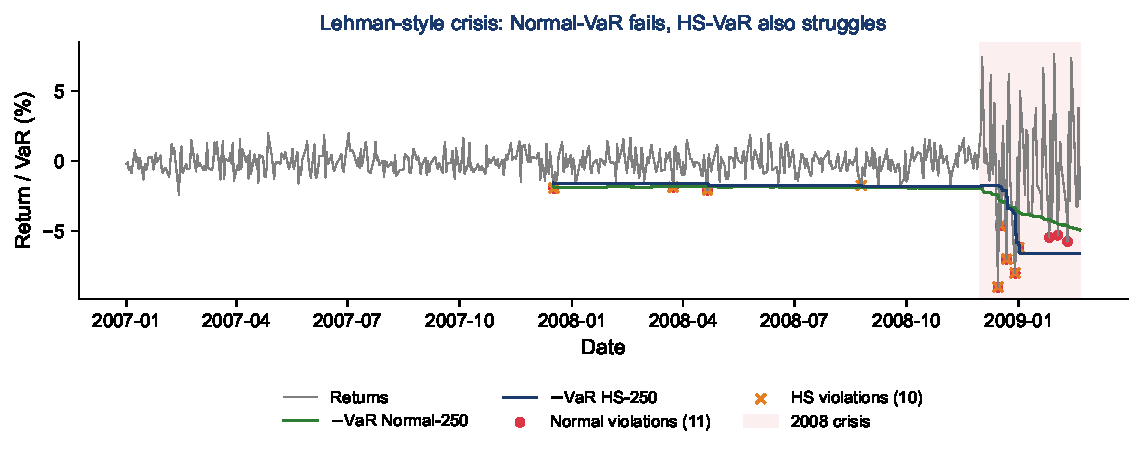
\includegraphics[width=\linewidth]{ch11_lehman_2008.pdf}
    \end{center}
    \end{column}
    \begin{column}{0.43\textwidth}
    \begin{block}{Datele Lehman (Q2 2008)}
    \begin{itemize}\setlength{\itemsep}{0pt}
        \item $\VaR^{10d}_{99\%}$ raportat: $\approx 100$M USD
        \item Pierderi efective sept.\ 2008: \textbf{miliarde}
        \item Excepții (10$\sigma$): \textbf{5 ori într-o lună} sub ipoteza Normală
    \end{itemize}
    \end{block}
    \begin{exampleblock}{Cauze identificate}
    \begin{itemize}\setlength{\itemsep}{0pt}
        \item Fereastră prea scurtă (250 zile bull market)
        \item Model risk: Normal pe MBS (mortgage-backed securities)
        \item Lichiditate ignorată
        \item Stress testing inadecvat
    \end{itemize}
    \end{exampleblock}
    \begin{alertblock}{Reforma}
    \begin{itemize}\setlength{\itemsep}{0pt}
        \item Basel III: Stressed VaR adăugat
        \item FRTB: ES + orizonturi de lichiditate
    \end{itemize}
    \end{alertblock}
    \end{column}
    \end{columns}
    \quantlet{SFM\_ch11\_lehman\_2008}{https://github.com/danpele/SFM/tree/main/Quantlets/Ch_11/SFM_ch11_lehman_2008}
    \end{cminipage}
\end{frame}

\begin{frame}[shrink=10]{Caz 3: Crypto crash 2022 --- VaR pe BTC}
    \begin{cminipage}{0.95\textwidth}
    \begin{columns}[T]
    \begin{column}{0.55\textwidth}
    \begin{center}
    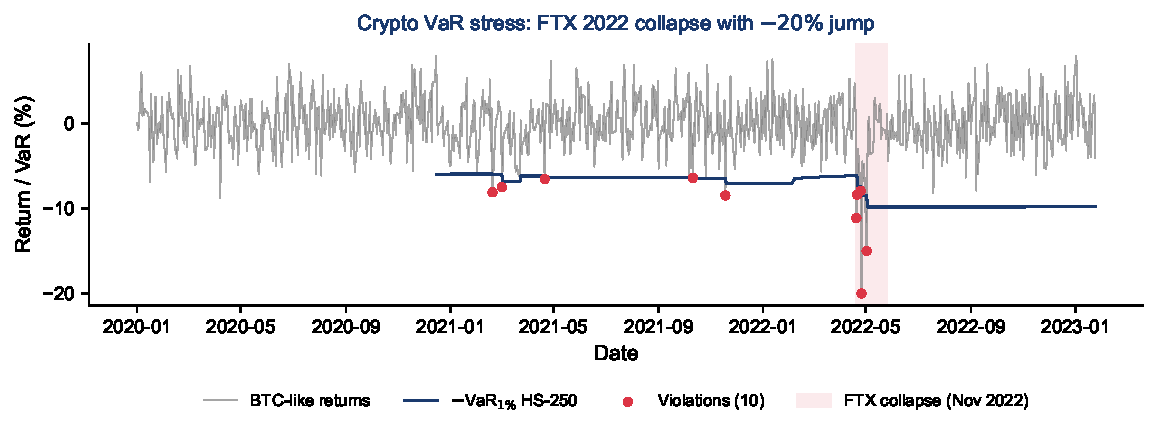
\includegraphics[width=\linewidth]{ch11_crypto_var.pdf}
    \end{center}
    \end{column}
    \begin{column}{0.43\textwidth}
    \begin{block}{Date BTC-USD 2020--2023}
    \begin{itemize}\setlength{\itemsep}{0pt}
        \item Vol anualizat: $\sigma \approx 60$--$80\%$ ($\approx 4$--$5\%$ zilnic)
        \item $\hat{\nu}$ (MLE): $\approx 3$ (cozi extrem de grele)
        \item Evenimente extreme 2022: Luna/Terra ($-99\%$), FTX ($-25\%$/zi), 3AC liquidations
    \end{itemize}
    \end{block}
    \begin{exampleblock}{VaR comparativ ($\sigma = 4\%$ zilnic)}
    \begin{itemize}\setlength{\itemsep}{0pt}
        \item $\VaR^{N}_{1\%} = 9{,}3\%$
        \item $\VaR^{t_3}_{1\%} = 17{,}5\%$ (+88\%)
        \item $\VaR^{HS}_{1\%} \approx 12$--$15\%$ (depinde de fereastră)
    \end{itemize}
    \end{exampleblock}
    \begin{alertblock}{Lecții}
    \begin{itemize}\setlength{\itemsep}{0pt}
        \item Crypto 24/7 $\Rightarrow$ ,,VaR zilnic'' ambiguu; liquidity gaps în weekend
        \item Recomandat: GARCH-$t$ + stress testing
    \end{itemize}
    \end{alertblock}
    \end{column}
    \end{columns}
    \quantlet{SFM\_ch11\_crypto\_var}{https://github.com/danpele/SFM/tree/main/Quantlets/Ch_11/SFM_ch11_crypto_var}
    \end{cminipage}
\end{frame}

\begin{frame}[shrink=10]{Caz 4: LTCM 1998 --- 4-SD events repetate}
\begin{cminipage}{0.95\textwidth}
\begin{columns}[T,onlytextwidth]
    \begin{column}{0.56\textwidth}
    \begin{center}
    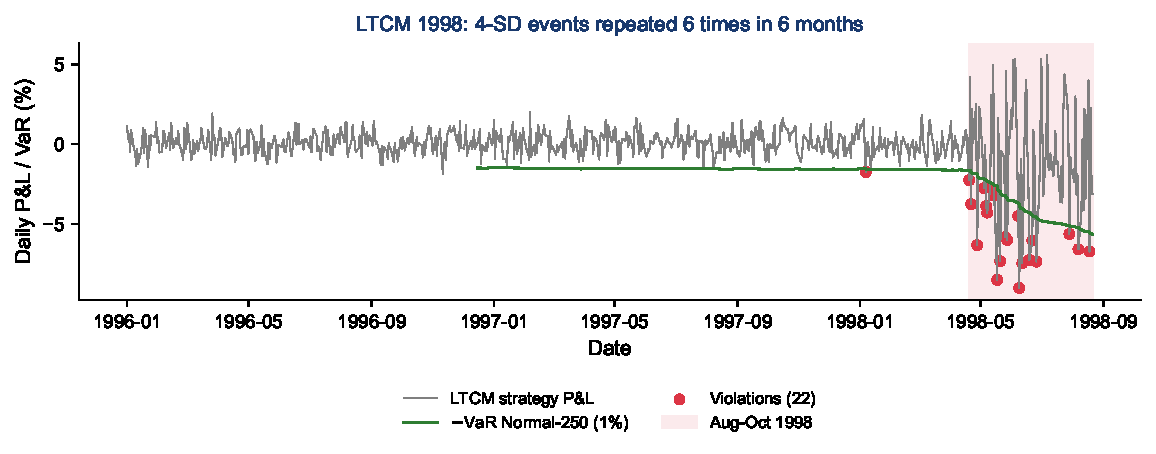
\includegraphics[width=\linewidth]{ch11_ltcm_1998.pdf}
    \end{center}
    \end{column}
    \begin{column}{0.43\textwidth}
    \begin{block}{Faptele}
    \begin{itemize}\setlength{\itemsep}{0pt}
        \item LTCM (Meriwether, Merton, Scholes): \$4{,}7 mld capital, leverage $\sim 30\times$, strategie \emph{relative value}
        \item Aug 1998: default Rusia, fugă spre calitate $\Rightarrow$ \textbf{spread-uri explodează} simultan global
        \item Pierdere \$4{,}6 mld în 4 luni; salvat de un consorțiu Fed
    \end{itemize}
    \end{block}
    \begin{alertblock}{Lecție VaR}
    \begin{itemize}\setlength{\itemsep}{0pt}
        \item Modelul: ,,4 SD events o dată la 1000 ani'' $\Rightarrow$ s-au repetat de 6 ori în 6 luni
        \item \textbf{Corelații instabile}: $\rho \to 1$ în criză $\Rightarrow$ diversificarea evaporă
        \item Reforma: \textbf{Stressed VaR} adăugat în Basel 2.5
    \end{itemize}
    \end{alertblock}
    \end{column}
\end{columns}
\quantlet{SFM\_ch11\_ltcm\_1998}{https://github.com/danpele/SFM/tree/main/Quantlets/Ch_11/SFM_ch11_ltcm_1998}
\end{cminipage}
\end{frame}

\begin{frame}[shrink=10]{Caz 5: COVID Martie 2020 --- ruptură de regim}
\begin{cminipage}{0.95\textwidth}
\begin{columns}[T,onlytextwidth]
    \begin{column}{0.56\textwidth}
    \begin{center}
    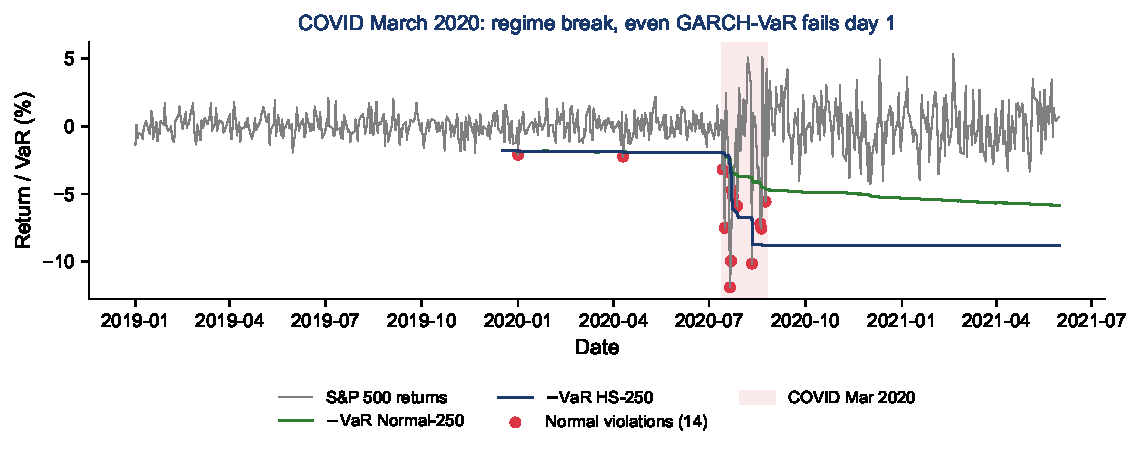
\includegraphics[width=\linewidth]{ch11_covid_2020.pdf}
    \end{center}
    \end{column}
    \begin{column}{0.43\textwidth}
    \begin{block}{Faptele}
    \begin{itemize}\setlength{\itemsep}{0pt}
        \item 16 martie 2020: S\&P 500 $-11{,}98\%$ (a 3-a cea mai mare pierdere din istorie)
        \item Volatilitate VIX: $14 \to 82$ în 4 săptămâni (cea mai rapidă creștere istorică)
        \item TLT (US Treasuries): paradoxal corelație pozitivă cu equity în panică inițială
    \end{itemize}
    \end{block}
    \begin{alertblock}{Lecție VaR}
    \begin{itemize}\setlength{\itemsep}{0pt}
        \item \textbf{Ruptură de regim}: niciun model rolling 250d nu o vede în ziua 1
        \item GARCH-VaR reacționează cu \textbf{1--2 zile întârziere}; HS reacționează după 250 zile
        \item \textbf{Filtered HS} și \textbf{realised volatility} s-au comportat mai bine în t+5
    \end{itemize}
    \end{alertblock}
    \end{column}
\end{columns}
\quantlet{SFM\_ch11\_covid\_2020}{https://github.com/danpele/SFM/tree/main/Quantlets/Ch_11/SFM_ch11_covid_2020}
\end{cminipage}
\end{frame}

\begin{frame}[shrink=10]{Caz 6: Archegos Martie 2021 --- risc de concentrare}
\begin{cminipage}{0.95\textwidth}
\begin{columns}[T,onlytextwidth]
    \begin{column}{0.56\textwidth}
    \begin{center}
    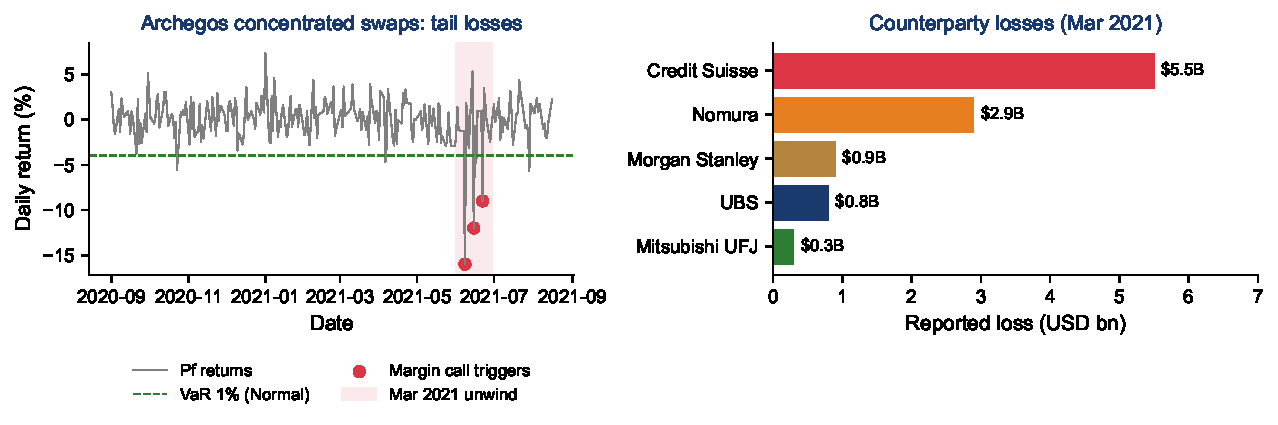
\includegraphics[width=\linewidth]{ch11_archegos_2021.pdf}
    \end{center}
    \end{column}
    \begin{column}{0.43\textwidth}
    \begin{block}{Faptele}
    \begin{itemize}\setlength{\itemsep}{0pt}
        \item Bill Hwang (Archegos): \$10 mld capital, \$50+ mld expunere via \textbf{TRS} (Total Return Swaps)
        \item Concentrat în câteva poziții (ViacomCBS, GSX, Discovery)
        \item Margin call lanț Mar 2021: \$10+ mld pierderi pentru prime broker-i (CS, Nomura)
    \end{itemize}
    \end{block}
    \begin{alertblock}{Lecție VaR}
    \begin{itemize}\setlength{\itemsep}{0pt}
        \item VaR standard \textbf{NU capturează concentrarea} pe nume single
        \item Prime broker-ii nu vedeau expunerea totală a clientului (TRS opace)
        \item Reforma: \textbf{single-name VaR limits}, raportare TRS-uri sub Basel
    \end{itemize}
    \end{alertblock}
    \end{column}
\end{columns}
\quantlet{SFM\_ch11\_archegos\_2021}{https://github.com/danpele/SFM/tree/main/Quantlets/Ch_11/SFM_ch11_archegos_2021}
\end{cminipage}
\end{frame}

\begin{frame}[shrink=10]{Caz 7: UK gilts Octombrie 2022 --- LDI pensions criză}
\begin{cminipage}{0.95\textwidth}
\begin{columns}[T,onlytextwidth]
    \begin{column}{0.56\textwidth}
    \begin{center}
    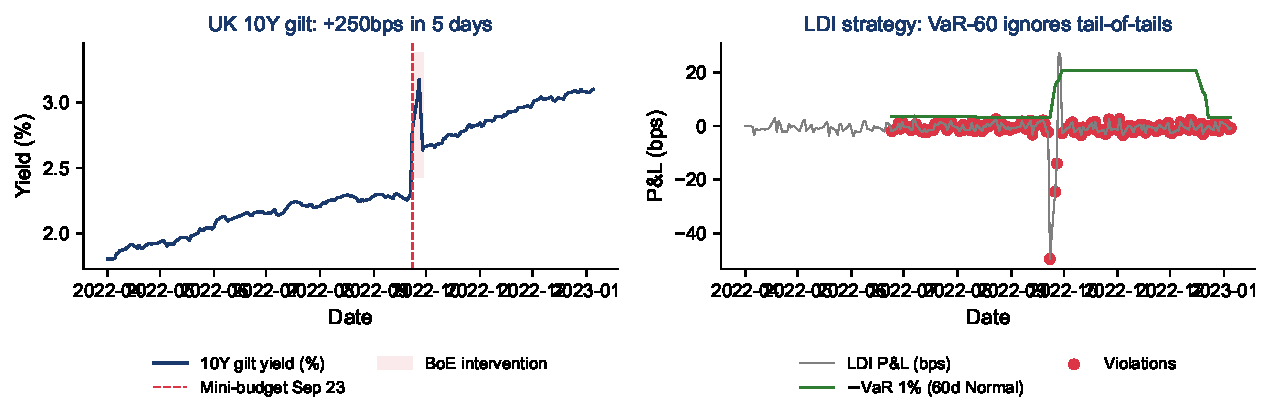
\includegraphics[width=\linewidth]{ch11_uk_gilts_2022.pdf}
    \end{center}
    \end{column}
    \begin{column}{0.43\textwidth}
    \begin{block}{Faptele}
    \begin{itemize}\setlength{\itemsep}{0pt}
        \item Mini-budget Truss (23 sept 2022): $\pm$£45 mld tăieri fiscale nefinanțate
        \item Yield 10Y gilt: $+250$ bps în 5 zile (mișcare istorică)
        \item LDI funds (£1.5 trn AUM): margin call în lanț, Bank of England intervine 28 sept
    \end{itemize}
    \end{block}
    \begin{alertblock}{Lecție VaR}
    \begin{itemize}\setlength{\itemsep}{0pt}
        \item LDI folosea \textbf{leverage $\sim 4\times$} pe duration; VaR cu fereastră 60 zile nu vedea coada
        \item Trigger \textbf{procyclic} (vânzare gilts $\to$ yield $\uparrow$ $\to$ margin call $\to$ vânzare)
        \item Reforma TPR: \textbf{liquidity buffer 250bps} și stress test cu $+400$bps
    \end{itemize}
    \end{alertblock}
    \end{column}
\end{columns}
\quantlet{SFM\_ch11\_uk\_gilts\_2022}{https://github.com/danpele/SFM/tree/main/Quantlets/Ch_11/SFM_ch11_uk_gilts_2022}
\end{cminipage}
\end{frame}

%=============================================================================
% EXERCIȚII PYTHON
%=============================================================================
\section{Exerciții Python}

\begin{frame}[shrink=10]{Exercițiu Python 1: Cele 4 metode standard}
\begin{cminipage}{0.95\textwidth}
    \begin{block}{Sarcină}
    \begin{enumerate}\setlength{\itemsep}{0pt}
        \item Descărcați randamentele zilnice ale SPY pe 2018--2025 cu \texttt{yfinance}
        \item Implementați 4 funcții pentru $\VaR_\alpha$ și $\ES_\alpha$: HS, Normal, Student-$t$, MC
        \item Aplicați la $\alpha \in \{5\%, 1\%, 0{,}1\%\}$ pe întregul eșantion
        \item Tabel comparativ: 4 metode $\times$ 3 niveluri
    \end{enumerate}
    \end{block}
    \vspace{0.15cm}
    \begin{alertblock}{Funcții cheie}
    \begin{itemize}\setlength{\itemsep}{0pt}
        \item \texttt{np.quantile(returns, alpha)} --- cuantila empirică (HS)
        \item \texttt{stats.norm.ppf(alpha)} --- cuantila Normală
        \item \texttt{stats.t.fit(returns)} --- MLE pentru $\nu$
        \item \texttt{stats.t.ppf(alpha, df=nu)} --- cuantila Student-$t$
        \item \texttt{np.random.normal(mu, sigma, M)} pentru MC
    \end{itemize}
    \end{alertblock}
    \quantlet{SFM\_ch11\_methods\_comparison}{https://github.com/danpele/SFM/tree/main/Quantlets/Ch_11/SFM_ch11_methods_comparison}
\end{cminipage}
\end{frame}

\begin{frame}[fragile,shrink=10]{Exercițiu Python 2: Rolling VaR + Backtesting Kupiec}
\begin{cminipage}{0.95\textwidth}
    \begin{block}{Sarcină}
    \begin{enumerate}\setlength{\itemsep}{0pt}
        \item Calculați rolling $\VaR_{1\%}^{HS}$ cu fereastră $W = 250$ pe randamentele SPY
        \item Construiți hit sequence $I_t = \mathbb{1}\{r_t < -\VaR_t\}$
        \item Vizualizați: randamentele $r_t$, $-\VaR_t$ și punctele de depășire
        \item Aplicați testul Kupiec POF: este modelul HS acceptat?
    \end{enumerate}
    \end{block}
    \vspace{0.15cm}
    \begin{alertblock}{Funcții cheie}
    \begin{itemize}\setlength{\itemsep}{0pt}
        \item \texttt{returns.rolling(250).quantile(0.01)} --- VaR rolling
        \item \texttt{hits = (returns < -var\_series).astype(int)}
        \item Statistica Kupiec:
        \begin{lstlisting}[language=Python]
x = hits.sum(); n = len(hits); p_hat = x/n
LR = -2*(x*np.log(alpha/p_hat) + (n-x)*np.log((1-alpha)/(1-p_hat)))
p_value = 1 - stats.chi2.cdf(LR, df=1)
        \end{lstlisting}
    \end{itemize}
    \end{alertblock}
    \quantlet{SFM\_ch11\_rolling\_var\_es}{https://github.com/danpele/SFM/tree/main/Quantlets/Ch_11/SFM_ch11_rolling_var_es}
\end{cminipage}
\end{frame}

\begin{frame}[fragile,shrink=10]{Exercițiu Python 3: GARCH-VaR cu inovații Student-$t$}
\begin{cminipage}{0.95\textwidth}
    \begin{block}{Sarcină}
    \begin{enumerate}\setlength{\itemsep}{0pt}
        \item Fit GARCH(1,1) cu inovații Student-$t$ pe randamentele BVB (BET sau SIF1) cu pachetul \texttt{arch}
        \item Extrageți $\hat{\sigma}_t$ și $\hat{\nu}$
        \item Calculați $\VaR^{GARCH-t}_{1\%}(t) = -\sigma_t \cdot \sqrt{(\nu-2)/\nu} \cdot t_\nu^{-1}(0{,}01)$
        \item Comparați cu $\VaR^{HS}$ pe aceeași perioadă --- unde diferă cel mai mult?
    \end{enumerate}
    \end{block}
    \vspace{0.15cm}
    \begin{exampleblock}{Cod schelet}
\begin{lstlisting}[language=Python]
from arch import arch_model
model = arch_model(returns*100, vol='Garch', p=1, q=1, dist='t')
fit = model.fit(disp='off')
sigma = fit.conditional_volatility / 100
nu = fit.params['nu']
z_alpha = stats.t.ppf(0.01, df=nu) * np.sqrt((nu-2)/nu)
VaR_garch = -sigma * z_alpha
\end{lstlisting}
    \end{exampleblock}
    \quantlet{SFM\_ch11\_garch\_var}{https://github.com/danpele/SFM/tree/main/Quantlets/Ch_11/SFM_ch11_garch_var}
\end{cminipage}
\end{frame}

\begin{frame}[shrink=10]{Exercițiu Python 4: Studiu de caz BVB --- portofoliu}
\begin{cminipage}{0.95\textwidth}
    \begin{block}{Sarcină}
    \begin{enumerate}\setlength{\itemsep}{0pt}
        \item Construiți un portofoliu echilibrat din 3 acțiuni BVB (e.g.\ TLV, SNG, BRD)
        \item Descărcați date prin \texttt{yfinance} (ticker \texttt{.RO}) pe 2020--2025
        \item Calculați $\VaR_{1\%}$ și $\ES_{1\%}$ prin toate cele 4 metode pe portofoliu
        \item Aplicați Basel Traffic Light: în ce zonă cade fiecare metodă?
        \item Calculați capitalul de risc de piață pentru poziție nominală de 1M RON
    \end{enumerate}
    \end{block}
    \vspace{0.15cm}
    \begin{alertblock}{Rezultate așteptate}
    \begin{itemize}\setlength{\itemsep}{0pt}
        \item HS: $\VaR_{1\%} \approx 3$--$5\%$ zilnic (depinde de fereastră și criza COVID)
        \item Normal: subestimează cu $\approx 30\%$ comparativ cu HS pe perioade volatile
        \item GARCH-$t$: cea mai bună acoperire (depășiri $\approx \alpha \cdot n$); zona \textcolor{Forest}{verde}
        \item Diferența pe BVB vs SPY: cozi mai grele, lichiditate mai mică $\Rightarrow$ ipoteza Normală mai problematică
    \end{itemize}
    \end{alertblock}
    \quantlet{SFM\_ch11\_bvb\_case}{https://github.com/danpele/SFM/tree/main/Quantlets/Ch_11/SFM_ch11_bvb_case}
\end{cminipage}
\end{frame}

\begin{frame}[fragile,shrink=10]{Exercițiu Python 5: Cornish-Fisher VaR}
\begin{cminipage}{0.95\textwidth}
    \begin{block}{Sarcină}
    \begin{enumerate}\setlength{\itemsep}{0pt}
        \item Estimați $\hat{s}$ (skewness) și $\hat{k}$ (excess kurtosis) ale randamentelor SPY
        \item Aplicați expansiunea Cornish-Fisher pentru $\VaR_{1\%}$ cu corecție de moment
        \item Comparați cu $\VaR^N$, $\VaR^t$ și $\VaR^{HS}$ pe aceeași perioadă
    \end{enumerate}
    \end{block}
    \begin{exampleblock}{Cod schelet}
\begin{lstlisting}[language=Python]
from scipy.stats import skew, kurtosis, norm
s, k = skew(returns), kurtosis(returns)
z = norm.ppf(0.01)
z_cf = z + (z**2 - 1)*s/6 + (z**3 - 3*z)*k/24 - (2*z**3 - 5*z)*s**2/36
VaR_cf = -(returns.mean() + returns.std() * z_cf)
\end{lstlisting}
    \end{exampleblock}
    \quantlet{SFM\_ch11\_cornish\_fisher}{https://github.com/danpele/SFM/tree/main/Quantlets/Ch_11/SFM_ch11_cornish_fisher}
\end{cminipage}
\end{frame}

\begin{frame}[fragile,shrink=10]{Exercițiu Python 6: Filtered Historical Simulation}
\begin{cminipage}{0.95\textwidth}
    \begin{block}{Sarcină (Hull-White 1998)}
    \begin{enumerate}\setlength{\itemsep}{0pt}
        \item Fit GARCH(1,1)-$t$ pe randamente; extrageți $\hat{\sigma}_t$ și $\hat{z}_t = r_t/\hat{\sigma}_t$
        \item $\VaR^{FHS}_\alpha(t+1) = -\hat{\sigma}_{t+1} \cdot Q_\alpha(\hat{z}_{1:t})$ unde $Q_\alpha$ e cuantila empirică a inovațiilor
        \item Comparați acoperirea cu HS clasic și GARCH-parametric prin Kupiec POF
    \end{enumerate}
    \end{block}
    \begin{exampleblock}{Cod schelet}
\begin{lstlisting}[language=Python]
fit = arch_model(r*100, vol='Garch', dist='t').fit(disp='off')
sigma = fit.conditional_volatility / 100
z_hat = r / sigma
sigma_next = sigma.iloc[-1] * np.sqrt(fit.params['alpha[1]'])
VaR_fhs = -sigma_next * np.quantile(z_hat.dropna(), 0.01)
\end{lstlisting}
    \end{exampleblock}
    \quantlet{SFM\_ch11\_filtered\_hs}{https://github.com/danpele/SFM/tree/main/Quantlets/Ch_11/SFM_ch11_filtered_hs}
\end{cminipage}
\end{frame}

\begin{frame}[fragile,shrink=10]{Exercițiu Python 7: GJR-GARCH cu efect de levier}
\begin{cminipage}{0.95\textwidth}
    \begin{block}{Sarcină}
    \begin{enumerate}\setlength{\itemsep}{0pt}
        \item Fit GJR-GARCH(1,1)-$t$: $\sigma^2_t = \omega + \alpha r^2_{t-1} + \gamma r^2_{t-1}\mathbf{1}\{r_{t-1}<0\} + \beta \sigma^2_{t-1}$
        \item Testați semnificația $\gamma$ vs zero (efect de levier prezent?)
        \item Calculați $\VaR^{GJR}_{1\%}$ și comparați cu GARCH simetric pe perioade volatile
    \end{enumerate}
    \end{block}
    \begin{exampleblock}{Cod schelet}
\begin{lstlisting}[language=Python]
from arch import arch_model
gjr = arch_model(r*100, vol='Garch', p=1, o=1, q=1, dist='t').fit(disp='off')
print(gjr.params)  # 'gamma[1]' = leverage coefficient
sigma_gjr = gjr.conditional_volatility / 100
z_alpha = stats.t.ppf(0.01, df=gjr.params['nu']) * np.sqrt((gjr.params['nu']-2)/gjr.params['nu'])
VaR_gjr = -sigma_gjr * z_alpha
\end{lstlisting}
    \end{exampleblock}
    \quantlet{SFM\_ch11\_gjr\_garch}{https://github.com/danpele/SFM/tree/main/Quantlets/Ch_11/SFM_ch11_gjr_garch}
\end{cminipage}
\end{frame}

\begin{frame}[fragile,shrink=10]{Exercițiu Python 8: Hill plot pentru indicele cozii}
\begin{cminipage}{0.95\textwidth}
    \begin{block}{Sarcină}
    \begin{enumerate}\setlength{\itemsep}{0pt}
        \item Calculați Hill estimator $\hat{\xi}_H(k) = \frac{1}{k}\sum_{i=1}^k \ln(X_{(i)}/X_{(k+1)})$ pentru $k = 10, \dots, n/4$
        \item Trasați \textbf{Hill plot}: $\hat{\xi}_H(k)$ vs $k$; căutați platoul de stabilitate
        \item Comparați cu $\hat{\xi}$ din GPD-MLE pe excese
    \end{enumerate}
    \end{block}
    \begin{exampleblock}{Cod schelet}
\begin{lstlisting}[language=Python]
losses = -returns.sort_values(ascending=False).values  # pierderi descendent
def hill(k, x): return np.mean(np.log(x[:k]/x[k]))
ks = np.arange(10, len(losses)//4)
xi_hat = np.array([hill(k, losses) for k in ks])
\end{lstlisting}
    \end{exampleblock}
    \quantlet{SFM\_ch11\_hill\_plot}{https://github.com/danpele/SFM/tree/main/Quantlets/Ch_11/SFM_ch11_hill_plot}
\end{cminipage}
\end{frame}

%=============================================================================
% ÎNTREBĂRI DE DISCUȚIE
%=============================================================================
\section{Întrebări de Discuție}

\begin{frame}[shrink=10]{Discuție 1: Alegerea metodei VaR în practică}
\begin{cminipage}{0.95\textwidth}
    \begin{itemize}\setlength{\itemsep}{0pt}
        \item \textbf{Scenariu:} Sunteți analist de risc la o bancă comercială cu trading book de 100M EUR. Trebuie să raportați VaR zilnic la regulatorul UE (CRR3).
        \item \textbf{Întrebări:}
    \end{itemize}
    \begin{enumerate}\setlength{\itemsep}{0pt}
        \item Care metodă (HS, Normal, Student-$t$, MC, GARCH-VaR) folosiți ca \textbf{principală}? De ce?
        \item Cum justificați alegerea ferestrei $W$ ($250$ vs $500$ vs $1000$ zile)? Trade-off?
        \item Pentru portofolii cu \textbf{opțiuni} (gamma negativ), de ce HS și Normal eșuează? Ce alegeți?
        \item Cum monitorizați \textbf{model risk}: cum verificați că modelul ales rămâne corect în timp?
        \item Sub FRTB (din 2025+), ce schimbări faceți în pipeline-ul de risk management?
    \end{enumerate}
\end{cminipage}
\end{frame}

\begin{frame}[shrink=10]{Discuție 2: Eșecul VaR --- lecții din 2008 și LTCM}
\begin{cminipage}{0.95\textwidth}
    \begin{itemize}\setlength{\itemsep}{0pt}
        \item \textbf{Scenariu:} LTCM (1998) folosea VaR Normal pe baza datelor 1990--1998. În august 1998, după criza rusească, au pierdut \$4{,}6 mld --- evenimente ,,4 SD'' s-au repetat de 6 ori în 6 luni.
        \item \textbf{Întrebări:}
    \end{itemize}
    \begin{enumerate}\setlength{\itemsep}{0pt}
        \item Care au fost cele 3 erori majore în modelarea VaR la LTCM?
        \item De ce ipoteza Normalei a fost critică? Cum ar fi arătat VaR-ul sub Student-$t_4$?
        \item Lehman (2008): banca raporta VaR de $\approx 100$M USD/zi, dar a pierdut zeci de miliarde. Cum se reconciliază?
        \item De ce GARCH-VaR nu a prevenit nici criza COVID (martie 2020)? Ce limitări fundamentale au modelele de risc?
        \item Stress testing (CCAR, DFAST) vs.\ VaR: complementare sau substituibile?
    \end{enumerate}
\end{cminipage}
\end{frame}

\begin{frame}[shrink=10]{Discuție 3: VaR vs ES sub FRTB --- impactul real}
\begin{cminipage}{0.95\textwidth}
    \begin{itemize}\setlength{\itemsep}{0pt}
        \item \textbf{Scenariu:} Tranziția Basel III $\to$ FRTB (2025+) înseamnă VaR 99\% $\to$ ES 97{,}5\% cu calibrare stresată.
        \item \textbf{Întrebări:}
    \end{itemize}
    \begin{enumerate}\setlength{\itemsep}{0pt}
        \item De ce ES la 97{,}5\% (nu 99\%)? Cum a fost calibrat regulatorul să dea capital similar sub Normală?
        \item Pe ce clase de active capitalul \textbf{crește} sub FRTB? (Indiciu: cozi grele)
        \item Backtesting ES: care e problema principală? Cum se rezolvă în practică (Acerbi--Szekely, ES/VaR ratio)?
        \item \textbf{Internal Models Approach (IMA)} vs.\ \textbf{Standardised Approach (SA)} sub FRTB: când conține fiecare?
        \item Cum afectează FRTB business model-ul băncilor cu trading book mare?
    \end{enumerate}
\end{cminipage}
\end{frame}

\begin{frame}[shrink=10]{Discuție 4: VaR pentru crypto și active emergente}
\begin{cminipage}{0.95\textwidth}
    \begin{itemize}\setlength{\itemsep}{0pt}
        \item \textbf{Scenariu:} Un client retail vă cere să cuantificați riscul investiției în Bitcoin (volatilitate $\sigma \approx 70\%$ anualizat) vs S\&P 500 ($\sigma \approx 16\%$).
        \item \textbf{Întrebări:}
    \end{itemize}
    \begin{enumerate}\setlength{\itemsep}{0pt}
        \item De ce VaR Normal este \textit{cu deosebire} inadecvat pentru BTC? (Distribuții, salturi, liquidity gaps)
        \item Calculați $\VaR_{1\%}$ zilnic pentru BTC sub Normal vs Student-$t_3$ --- factor de creștere?
        \item BTC se tranzacționează 24/7: cum interpretați VaR-ul ,,zilnic''? Care e orizontul natural?
        \item Sub MiFID II (PRIIPs): cum raportați VaR retail (97{,}5\%, holding period)? Ce e ,,Summary Risk Indicator''?
        \item Crypto crashes (FTX 2022, Terra/Luna): VaR ex-ante vs.\ pierderi ex-post? Ce metodă ar fi prezis?
    \end{enumerate}
\end{cminipage}
\end{frame}

\begin{frame}[shrink=10]{Discuție 5: AI/LLM în managementul riscului}
\begin{cminipage}{0.95\textwidth}
    \begin{itemize}\setlength{\itemsep}{0pt}
        \item \textbf{Scenariu:} Echipa de risc al băncii primește presiune să folosească LLM-uri (GPT-4, Claude) pentru rapoarte VaR săptămânale. Riscul ,,model-on-model''.
        \item \textbf{Întrebări:}
    \end{itemize}
    \begin{enumerate}\setlength{\itemsep}{0pt}
        \item Care sunt cele \textbf{3 riscuri majore} ale folosirii LLM-urilor pentru calculele VaR? (Hallucination, drift, auditabilitate)
        \item Cum se încadrează asta în \textbf{SR 11-7} (Federal Reserve Model Risk) și \textbf{EBA Model Risk Guidelines}?
        \item Acceptabil să folosiți LLM pentru: documentație? Cod prototip? Calcul direct? Backtest interpretation?
        \item Cum implementați \textbf{control-by-design}: validare independentă, replicabilitate (seed), audit trail?
        \item \textbf{AI Act (UE 2024)}: LLM-urile în risc bancar sunt ,,high-risk AI''? Ce obligații implică?
    \end{enumerate}
\end{cminipage}
\end{frame}

\begin{frame}[shrink=10]{Discuție 6: Climate risk și ESG VaR}
\begin{columns}[T,onlytextwidth]
    \begin{column}{0.55\textwidth}
    \begin{center}
    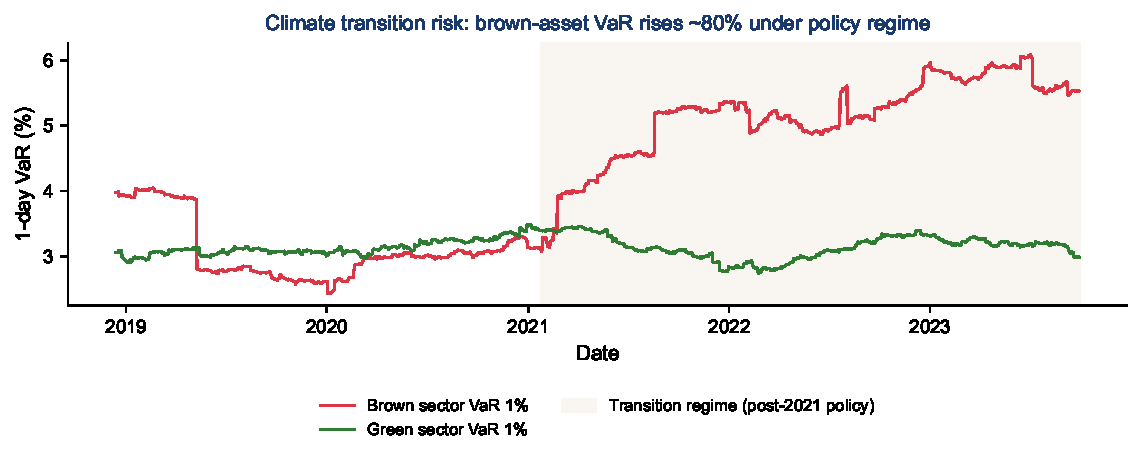
\includegraphics[width=\linewidth]{ch11_climate_var.pdf}
    \end{center}
    \end{column}
    \begin{column}{0.43\textwidth}
    \begin{cminipage}{\linewidth}
    \begin{itemize}\setlength{\itemsep}{0pt}
        \item \textbf{Scenariu:} Portofoliu cu expunere ,,brown'' (energie fosilă) și ,,green'' (regenerabile). Regimul post-2021 schimbă DGP.
    \end{itemize}
    \begin{enumerate}\setlength{\itemsep}{0pt}
        \item De ce VaR istoric subestimează \textbf{transition risk}? (Schimbare structurală în DGP)
        \item Cum integrați \textbf{scenarii NGFS} (Net Zero, Disorderly, Hot House World) în calculele VaR?
        \item \textbf{ECB Climate Stress Test (2022)}: ce metodologie a folosit? Ce a dezvăluit pentru băncile RO?
        \item Concept de \textbf{stranded assets} --- cum se traduce într-un haircut VaR?
        \item \textbf{TCFD / CSRD}: implicații pentru raportarea VaR ESG-adjusted
    \end{enumerate}
    \end{cminipage}
    \end{column}
\end{columns}
\end{frame}

%=============================================================================
% EXERCIȚII CU ASISTENȚĂ AI
%=============================================================================
\section{Exerciții cu asistență AI}

\begin{frame}[shrink=10]{Exercițiu AI 1: Prompt Engineering pentru VaR}
    \begin{cminipage}{0.95\textwidth}
    \begin{block}{Cerință}
    \begin{itemize}\setlength{\itemsep}{0pt}
        \item Formulați un prompt LLM pentru un \textbf{pipeline complet} VaR + backtesting; specificați: data, metode, niveluri, fereastră, teste, format output
    \end{itemize}
    \end{block}
    \begin{exampleblock}{Exemplu de prompt bun}
    \begin{itemize}\setlength{\itemsep}{0pt}
        \item \textit{,,Scrie un script Python care: (1) descarcă AAPL 2018--2025 cu yfinance; (2) calculează rolling VaR și ES la $\alpha = 1\%$, fereastră 250, prin HS, Normal, GARCH(1,1)-$t$ (\texttt{arch}); (3) aplică Kupiec POF și Christoffersen IC; (4) clasifică în zonele Basel; (5) vizualizează randamente, $-\VaR$ și depășirile pe 3 subgrafice. Format: PEP-8, comentarii RO.''}
    \end{itemize}
    \end{exampleblock}
    \begin{alertblock}{Întrebări de reflecție}
    \begin{itemize}\setlength{\itemsep}{0pt}
        \item Folosește formula corectă pentru cuantila Student-$t$ standardizată ($\sqrt{(\nu-2)/\nu}$)?
        \item Tratează NaN-urile la începutul ferestrei și zonele Basel pe ultimele 250 zile?
    \end{itemize}
    \end{alertblock}
    \end{cminipage}
\end{frame}

\begin{frame}[shrink=10]{Exercițiu AI 2: Verificarea codului generat}
\begin{cminipage}{0.95\textwidth}
    \begin{block}{Cerință}
    \begin{itemize}\setlength{\itemsep}{0pt}
        \item Cereți LLM-ului: \textit{,,Scrie o funcție Python pentru testul Christoffersen Conditional Coverage''}
        \item Rulați codul --- funcționează? Statistica este corect calculată?
    \end{itemize}
    \end{block}
    \vspace{0.1cm}
    \begin{alertblock}{Checklist de verificare}
    \begin{itemize}\setlength{\itemsep}{0pt}
        \item Contorul $n_{ij}$ este calculat corect (atenție la \texttt{shift(1)} și \texttt{dropna()})?
        \item Edge cases: $n_{11} = 0$ sau $n_{00} = 0$ (probabilități de tranziție 0 sau 1)? Codul protejează cu \texttt{np.log} pe 0?
        \item Statistica $LR_{CC} = LR_{POF} + LR_{IC}$ este suma corectă a celor două?
        \item Distribuția de referință este $\chi^2_2$ (nu $\chi^2_1$)?
    \end{itemize}
    \end{alertblock}
    \vspace{0.1cm}
    \begin{exampleblock}{Obiectiv pedagogic}
    \begin{itemize}\setlength{\itemsep}{0pt}
        \item LLM-urile generează frecvent cod cu \textbf{eroare la edge cases} (probabilități 0/1, ferestre incomplete)
        \item În risc, o eroare în backtesting $\Rightarrow$ decizie greșită de zonă Basel $\Rightarrow$ capital greșit
        \item \textbf{Regulă de aur}: \textit{nu raporta niciodată un test statistic fără să-l verifici manual pe un caz cunoscut}
    \end{itemize}
    \end{exampleblock}
\end{cminipage}
\end{frame}

\begin{frame}[shrink=10]{Exercițiu AI 3: Critică unui raport de risc generat de AI}
    \begin{cminipage}{0.95\textwidth}
    \begin{block}{Cerință}
    \begin{itemize}\setlength{\itemsep}{0pt}
        \item Un coleg vă trimite un raport de risc generat cu AI care afirmă: \textit{,,Portofoliul are $\VaR_{99\%} = 50.000$ EUR. Sub ipoteza Normalei, capitalul Basel necesar este $3 \times 50.000 = 150.000$ EUR.''}
        \item \textbf{Sarcina}: identificați \textbf{3 erori sau omisiuni} critice în acest raport
    \end{itemize}
    \end{block}
    \vspace{0.1cm}
    \begin{exampleblock}{Erori așteptate}
    \begin{itemize}\setlength{\itemsep}{0pt}
        \item \textbf{Eroare 1 --- orizont}: VaR Basel este la \textbf{10 zile}, nu 1 zi $\Rightarrow$ scalare $\sqrt{10}$
        \item \textbf{Eroare 2 --- multiplier}: $m = 3$ este \textbf{minimul} (zona verde); după backtesting poate crește la 3{,}40--4
        \item \textbf{Eroare 3 --- ipoteză Normală}: dacă portofoliul are cozi grele, $\VaR^{N}$ subestimează cu 30--60\%
        \item \textbf{Omisiuni}: nivelul exact ($99\%$ sau $97{,}5\%$?), perioada de calibrare, lichiditate, Stressed VaR
        \item \textbf{Capital corect}: $\approx 3{,}5 \cdot \sqrt{10} \cdot 50.000 \cdot 1{,}3 \approx 720.000$ EUR (factor $\sim 5\times$)
    \end{itemize}
    \end{exampleblock}
    \begin{alertblock}{Lecția pedagogică}
    \begin{itemize}\setlength{\itemsep}{0pt}
        \item LLM-urile produc rapoarte plauzibile sintactic, dar omit \textbf{detalii regulatoare} critice
        \item \textbf{Regulă}: în risc, fiecare cifră trebuie să specifice $\alpha$, orizontul, distribuția și fereastra
    \end{itemize}
    \end{alertblock}
    \end{cminipage}
\end{frame}

\begin{frame}[shrink=10]{Exercițiu AI 4: Debugging unei zone Basel cu AI}
    \begin{cminipage}{0.95\textwidth}
    \begin{block}{Cerință}
    \begin{itemize}\setlength{\itemsep}{0pt}
        \item Modelul VaR a primit \textbf{12 depășiri} în 250 zile (99\%) $\Rightarrow$ zona \textcolor{Crimson}{roșie}; cereți LLM-ului diagnostic + acțiuni corective
    \end{itemize}
    \end{block}
    \begin{exampleblock}{Prompt structurat}
    \begin{itemize}\setlength{\itemsep}{0pt}
        \item \textit{,,Am 12 depășiri VaR 99\% în 250 zile, zonă roșie. Hit sequence CSV (date, $r_t$, $\VaR_t$, $I_t$). Diagnostichează: (a) acoperire necondițională sau clustering (Kupiec POF + Christoffersen IC); (b) ce perioadă a generat majoritatea depășirilor; (c) ce metodă alternativă recomanzi (GARCH-$t$, FHS, EVT). Justifică pe date.''}
    \end{itemize}
    \end{exampleblock}
    \begin{alertblock}{Checklist verificare răspuns AI}
    \begin{itemize}\setlength{\itemsep}{0pt}
        \item Calculează \textbf{ambele} statistici (POF + IC)? Identifică \textbf{clustering} (e.g., martie 2020)?
        \item Recomandă metodă compatibilă cu volumul de date (EVT pentru cuantile mici)?
        \item Nu inventează hiperparametri fără justificare; tratează \textbf{model risk} (suprapunere calibrare/backtest)?
    \end{itemize}
    \end{alertblock}
    \end{cminipage}
\end{frame}

\begin{frame}[shrink=10]{Exercițiu AI 5: Design de scenarii de stres cu AI}
    \begin{cminipage}{0.95\textwidth}
    \begin{block}{Cerință}
    \begin{itemize}\setlength{\itemsep}{0pt}
        \item Cereți LLM-ului să propună \textbf{5 scenarii istorice} pentru stress testing al unui portofoliu BVB
        \item Pentru fiecare: șocuri pe rate, FX, equity; corelații în criză; orizont; calibrare istorică
    \end{itemize}
    \end{block}
    \begin{exampleblock}{Prompt structurat (CCAR-style)}
    \begin{itemize}\setlength{\itemsep}{0pt}
        \item \textit{,,Portofoliu BVB: 40\% bănci, 30\% energie, 20\% utilities, 10\% TLV. Propune 5 scenarii adverse cu probabilitate 1/25 ani. Pentru fiecare: (a) trigger macro (gaz, contagiune, default suveran); (b) șocuri concrete (RON/EUR, ROBOR, BET); (c) corelație stresată; (d) impact estimat P\&L; (e) acțiuni mitigare.''}
    \end{itemize}
    \end{exampleblock}
    \begin{alertblock}{Verificare independentă}
    \begin{itemize}\setlength{\itemsep}{0pt}
        \item Scenariile sunt \textbf{plauzibile} dar suficient de \textbf{severe} (cap la $-3$ std nu e ,,stres'')?
        \item LLM-ul propune corelații \textbf{stresate} (la $\rho \to 1$ în criză) sau folosește $\rho$ istoric naïv?
        \item Sunt scenariile \textbf{decorelate} între ele (nu doar variații pe același temă)?
    \end{itemize}
    \end{alertblock}
    \end{cminipage}
\end{frame}

\begin{frame}[shrink=10]{Exercițiu AI 6: Multi-LLM consensus pe raport de risc}
    \begin{cminipage}{0.95\textwidth}
    \begin{block}{Cerință}
    \begin{itemize}\setlength{\itemsep}{0pt}
        \item Trimiteți același prompt VaR la \textbf{3 LLM-uri} diferite (Claude, GPT-4, Gemini); comparați outputs
        \item Identificați unde converg și unde divergă în concluzii și recomandări
    \end{itemize}
    \end{block}
    \begin{exampleblock}{Protocol experimental}
    \begin{itemize}\setlength{\itemsep}{0pt}
        \item Prompt: \textit{,,Analizați hit sequence atașat (CSV); recomandați model. Răspuns: 200 cuvinte, structurat: (1) diagnostic; (2) test stat; (3) recomandare cu justificare cantitativă.''}
        \item Compară: \textbf{convergența} diagnosticului; \textbf{divergența} testelor folosite; \textbf{calitatea} recomandării
    \end{itemize}
    \end{exampleblock}
    \begin{alertblock}{Lecția pedagogică}
    \begin{itemize}\setlength{\itemsep}{0pt}
        \item Niciun LLM nu este oracol; \textbf{consensul} reduce hallucination dar nu elimină erorile sistematice
        \item Folosiți LLM-urile ca \textbf{junior analist} (rapid + greșeli previzibile), nu ca expert independent
    \end{itemize}
    \end{alertblock}
    \end{cminipage}
\end{frame}

%=============================================================================
% REZUMAT
%=============================================================================
\section{Rezumat}

\begin{frame}[shrink=10]{Concluzii și pași următori}
\begin{cminipage}{0.95\textwidth}
    \begin{enumerate}\setlength{\itemsep}{0pt}
        \item \textbf{VaR} este cuantila distribuției pierderilor: prag depășit cu probabilitate $\alpha$
        \item \textbf{ES} este media pierderilor în coadă --- distinge severitatea, nu doar pragul
        \item \textbf{4 metode standard}: HS (non-parametrică), Normal, Student-$t$, MC --- alegerea depinde de date și orizont
        \item \textbf{GARCH-VaR} răspunde la șocuri în 1--2 zile; HS lag $W$ zile
        \item \textbf{Subaditivitatea} eșuează la VaR pe distribuții non-eliptice $\Rightarrow$ ES coerentă
        \item \textbf{Backtesting} obligatoriu: Kupiec POF (frecvență) + Christoffersen IC (clustering)
        \item \textbf{Basel Traffic Light}: 0--4 verde, 5--9 galben (penalizare), $\geq 10$ roșu (model respins)
        \item \textbf{FRTB} (2025+): trecere VaR 99\% $\to$ ES 97{,}5\% sub calibrare stresată
    \end{enumerate}

    \vspace{0.3cm}
    \begin{block}{Următorul Seminar}
        Studiu de caz integrat: portofoliu cu acțiuni BVB, măsurarea riscului end-to-end, raport tip RWA
    \end{block}
\end{cminipage}
\end{frame}

\begin{frame}[shrink=10]{Temă pentru acasă}
\begin{cminipage}{0.95\textwidth}
    \begin{block}{Obiectiv}
    Analizați riscul de piață pentru un portofoliu multi-activ pe orizont de 1 zi.
    \end{block}
    \begin{enumerate}\setlength{\itemsep}{0pt}
        \item Descărcați date 2019--2025 pentru: un indice (SPY), o acțiune BVB (TLV.RO) și BTC-USD
        \item Calculați $\VaR_{1\%}$ și $\ES_{1\%}$ pe fiecare activ prin: HS ($W=250$), Normal, Student-$t$ MLE
        \item Construiți portofoliu echilibrat (1/3 fiecare) cu poziție nominală 1M EUR
        \item Calculați rolling $\VaR^{HS}_{1\%}$ pe portofoliu și hit sequence
        \item Aplicați testele Kupiec POF și Christoffersen IC --- raportați $LR$ și $p$-value
        \item Determinați zona Basel Traffic Light și capitalul de risc de piață ($m \cdot \VaR^{10d}$)
        \item Calculați ES Acerbi--Szekely backtest pentru ES-ul portofoliului
        \item \textbf{Întrebare}: Care activ are cele mai grele cozi? Cum ați justifica alegerea metodei recomandate pentru fiecare?
    \end{enumerate}
    \quantlet{SFM\_ch11\_bvb\_case}{https://github.com/danpele/SFM/tree/main/Quantlets/Ch_11/SFM_ch11_bvb_case}
\end{cminipage}
\end{frame}

\begin{frame}[shrink=10]{Glosar de terminologie}
\begin{cminipage}{0.95\textwidth}
\begin{block}{Concepte cheie}
\begin{itemize}\setlength{\itemsep}{0pt}
    \item \textbf{VaR$_\alpha$} --- cuantila $\alpha$ a pierderilor; \textbf{ES$_\alpha$} = $\mathbb{E}[L \mid L \geq \VaR_\alpha]$, media coadei
    \item \textbf{Coerență (Artzner)}: monotonie + invarianță translațională + omogenitate + subaditivitate
    \item \textbf{Hit sequence} $I_t = \mathbf{1}\{r_t < -\VaR_t\}$; \textbf{Backtesting} = test out-of-sample
\end{itemize}
\end{block}
\begin{block}{Metode}
\begin{itemize}\setlength{\itemsep}{0pt}
    \item \textbf{HS}, \textbf{Normal}, \textbf{Student-$t$}, \textbf{MC} (4 metode standard)
    \item \textbf{FHS} (Hull-White 1998): HS pe inovații GARCH; \textbf{Cornish-Fisher}: corecție skew/kurt
    \item \textbf{EVT POT} (GPD) și \textbf{Block Maxima} (GEV); \textbf{GJR-GARCH}: leverage effect
\end{itemize}
\end{block}
\begin{block}{Backtesting și reglementare}
\begin{itemize}\setlength{\itemsep}{0pt}
    \item \textbf{Kupiec POF} (frecvență), \textbf{Christoffersen IC/CC} (clustering), \textbf{Lopez} (magnitudine)
    \item \textbf{Basel Traffic Light}: 0--4 verde, 5--9 galben, $\geq 10$ roșu (250 zile, 99\%); \textbf{FRTB} (2025+): VaR$\to$ES 97{,}5\%
\end{itemize}
\end{block}
\end{cminipage}
\end{frame}

\begin{frame}[shrink=10]{Roadmap pentru aprofundare}
\begin{cminipage}{0.95\textwidth}
\begin{block}{Nivelul 1 --- Fundamente (anul III)}
\begin{itemize}\setlength{\itemsep}{0pt}
    \item Cele 4 metode standard (HS, Normal, Student-$t$, MC) + backtesting Kupiec
    \item Citiți: Jorion (2007) cap. 5--7; replicați quantlet-urile \texttt{SFM\_ch11\_method\_*}
\end{itemize}
\end{block}
\begin{block}{Nivelul 2 --- Avansate (master)}
\begin{itemize}\setlength{\itemsep}{0pt}
    \item GARCH-VaR / GJR / Filtered HS / Cornish-Fisher; backtesting Christoffersen CC + Lopez
    \item EVT (POT cu GPD; Block Maxima cu GEV; Hill estimator); ES coerent, Acerbi-Szekely
    \item Citiți: McNeil-Frey-Embrechts (2015) cap. 7--10; quantlet-urile \texttt{SFM\_ch11\_filtered\_hs}, \texttt{SFM\_ch11\_gjr\_garch}, \texttt{SFM\_ch11\_hill\_plot}
\end{itemize}
\end{block}
\begin{block}{Nivelul 3 --- Cercetare/Practică (PhD / industrie)}
\begin{itemize}\setlength{\itemsep}{0pt}
    \item Multivariate VaR (copule, factor models, DCC-GARCH); risc sistemic (CoVaR, MES)
    \item FRTB \emph{Internal Models Approach}: liquidity horizons, non-modellable risk factors, P\&L attribution
    \item Climate VaR / transition risk; Quantum Monte Carlo; ML pentru hit sequence prediction
\end{itemize}
\end{block}
\end{cminipage}
\end{frame}

\begin{frame}[shrink=10]{Bibliografie selectivă}
\begin{cminipage}{0.95\textwidth}
\begin{block}{Cărți și articole fundamentale}
\begin{itemize}\setlength{\itemsep}{0pt}
    \item \textbf{Artzner, Delbaen, Eber, Heath (1999)} --- ,,Coherent Measures of Risk'' --- axiomatic
    \item \textbf{McNeil, Frey, Embrechts (2015)} --- \textit{Quantitative Risk Management} (carte de referință)
    \item \textbf{Acerbi, Tasche (2002)} --- ,,On the coherence of expected shortfall''
    \item \textbf{Christoffersen (1998)} --- ,,Evaluating Interval Forecasts'' (testul IC/CC)
    \item \textbf{Kupiec (1995)} --- ,,Techniques for Verifying the Accuracy of Risk Models''
    \item \textbf{Jorion (2007)} --- \textit{Value at Risk: The New Benchmark} (Ed. 3)
\end{itemize}
\end{block}
\vspace{0.15cm}
\begin{block}{Documente regulatoare}
\begin{itemize}\setlength{\itemsep}{0pt}
    \item \textbf{BCBS (2019)} --- ,,Minimum capital requirements for market risk'' (FRTB final)
    \item \textbf{BCBS (1996)} --- ,,Supervisory framework for the use of backtesting''
    \item \textbf{CRR3 / CRD VI (UE 2024)} --- transpunerea Basel III final în dreptul Uniunii
\end{itemize}
\end{block}
\end{cminipage}
\end{frame}

{
\setbeamertemplate{headline}{}
\setbeamertemplate{footline}{}
\begin{frame}{}
    \vspace{1.5cm}
    \begin{center}
    {\LARGE\textcolor{IDAred}{Vă mulțumesc!}} \quad {\large\textcolor{MainBlue}{Întrebări?}}

    \vspace{1.0cm}

    Materialele seminarului sunt disponibile la: \href{https://danpele.github.io/SFM/}{\texttt{https://danpele.github.io/SFM/}}

    \vspace{0.3cm}

    \href{https://quantlet.com}{\raisebox{-0.15em}{
\includegraphics[height=0.8em]{ql_logo.png}} Quantlet} \quad
    \href{https://quantinar.com}{\raisebox{-0.15em}{
\includegraphics[height=0.8em]{qr_logo.png}} Quantinar}

    \vspace{0.3cm}

    {\small\href{https://colab.research.google.com/github/danpele/SFM/blob/main/Quantlets/Ch_11/SFM_ch11_methods_comparison/SFM_ch11_methods_comparison.ipynb}{\raisebox{-0.15em}{
\includegraphics[height=0.8em]{ql_logo.png}} Open in Google Colab}}
    \end{center}
\end{frame}
}

\end{document}
